\documentclass[12pt,a4paper]{article}

% Packages
\usepackage[utf8]{inputenc}
\usepackage[vietnamese]{babel}
\usepackage{geometry}
\usepackage{graphicx}
\usepackage{hyperref}
\usepackage{listings}
\usepackage{xcolor}
\usepackage{amsmath}
\usepackage{float}
\usepackage{caption}
\usepackage{subcaption}
\usepackage{enumitem}
\usepackage{fancyhdr}
\usepackage{titlesec}
\usepackage{tocloft}

% Page geometry
\geometry{
    left=3cm,
    right=2cm,
    top=2.5cm,
    bottom=2.5cm
}

% Header and footer
\pagestyle{fancy}
\fancyhf{}
\fancyhead[L]{Vending Machine System}
\fancyhead[R]{STM32 Project Report}
\fancyfoot[C]{\thepage}

% Code listing style
\lstdefinestyle{cstyle}{
    language=C,
    basicstyle=\ttfamily\small,
    keywordstyle=\color{blue}\bfseries,
    commentstyle=\color{gray}\itshape,
    stringstyle=\color{red},
    numbers=left,
    numberstyle=\tiny\color{gray},
    stepnumber=1,
    numbersep=8pt,
    backgroundcolor=\color{white},
    showspaces=false,
    showstringspaces=false,
    showtabs=false,
    frame=single,
    rulecolor=\color{black},
    tabsize=4,
    captionpos=b,
    breaklines=true,
    breakatwhitespace=false,
    escapeinside={(*@}{@*)}
}

\lstset{style=cstyle}

% Hyperref setup
\hypersetup{
    colorlinks=true,
    linkcolor=black,
    citecolor=blue,
    urlcolor=blue,
    pdftitle={Vending Machine Technical Report},
    pdfauthor={Nguyen Hung Thinh, Le The Loc, Tran Doan Hoang Lam}
}

% Title information
\title{
    \Large\textbf{TRƯỜNG ĐẠI HỌC BÁCH KHOA TP.HCM}\\
    \large Khoa Khoa học và Kỹ thuật Máy tính\\
    \vspace{2cm}
    \rule{\textwidth}{1.5pt}\\
    \vspace{0.5cm}
    \Huge\textbf{HỆ THỐNG MÁY BÁN HÀNG TỰ ĐỘNG}\\
    \Large\textbf{Báo cáo Kỹ thuật}\\
    \vspace{0.3cm}
    \Large Đồ án Thiết kế Luận lý với Vi điều khiển STM32\\
    \rule{\textwidth}{1.5pt}\\
}

\author{
    \textbf{Nhóm tác giả:}\\
    Nguyễn Hưng Thịnh\\
    Lê Thế Lộc\\
    Trần Doãn Hoàng Lâm\\
    \vspace{1cm}\\
    \textbf{Đơn vị:}\\
    Trường Đại học Bách Khoa TP.HCM (HCMUT)\\
}

\date{Ngày 20 tháng 12 năm 2025}

\begin{document}

% Title page
\maketitle
\thispagestyle{empty}
\newpage

% Abstract
\begin{abstract}
Báo cáo kỹ thuật này trình bày quá trình thiết kế và hiện thực hệ thống máy bán hàng tự động thông minh sử dụng vi điều khiển STM32F103C8T6. Hệ thống được thiết kế đặc biệt để bán các vật phẩm trong trò chơi (Trang phục đội tuyển SKT trong Liên Minh Huyền Thoại) và có các tính năng như tự động phát hiện khách hàng thông qua cảm biến siêu âm, giao diện LCD tương tác với bàn phím, quản lý kho hàng không bay hơi sử dụng bộ nhớ Flash, xử lý thanh toán toàn diện và chế độ quản trị bảo mật để kiểm soát kho hàng. Dự án minh họa các ứng dụng thực tế của nguyên lý hệ thống nhúng bao gồm thiết kế máy trạng thái hữu hạn, giao tiếp ngoại vi, điều khiển thời gian thực và lưu trữ dữ liệu. Việc hiện thực sử dụng thư viện STM32 HAL và bao gồm các trình điều khiển tùy chỉnh cho giao tiếp LCD I2C, quét bàn phím ma trận 4x4 và đo khoảng cách siêu âm HC-SR04. Các tính năng chính bao gồm tự động bật nguồn thông qua phát hiện khách hàng, xử lý giao dịch đa trạng thái với xử lý lỗi và lưu trữ kho hàng dựa trên bộ nhớ Flash qua các chu kỳ nguồn.
\end{abstract}

\newpage

% Table of contents
\renewcommand{\contentsname}{Mục lục}
\tableofcontents
\newpage

% Main content
\section{Giới thiệu}

\subsection{Bối cảnh và Động lực}

Máy bán hàng tự động đại diện cho một ứng dụng quan trọng của hệ thống nhúng trong tự động hóa bán lẻ hiện đại. Các hệ thống này đòi hỏi sự tích hợp phần cứng-phần mềm đáng tin cậy, phản hồi thời gian thực với đầu vào của người dùng và cơ chế xử lý lỗi mạnh mẽ. Thị trường máy bán hàng tự động toàn cầu tiếp tục mở rộng, với nhu cầu ngày càng tăng về các giải pháp bán lẻ tự động thông minh, thân thiện với người dùng có thể hoạt động tự chủ với sự can thiệp tối thiểu của con người.

Dự án này hiện thực một hệ thống máy bán hàng tự động toàn diện sử dụng vi điều khiển STM32F103C8T6, hướng đến thị trường vật phẩm game bằng cách bán các trang phục đội tuyển SKT trong Liên Minh Huyền Thoại. Việc lựa chọn lĩnh vực sản phẩm cụ thể này cho phép minh họa các nguyên tắc quản lý kho hàng trong khi vẫn duy trì sự hấp dẫn đối với cộng đồng game thủ. Hệ thống giải quyết một số thách thức chính trong thiết kế hệ thống nhúng bao gồm quản lý trạng thái, giao tiếp ngoại vi, lưu trữ dữ liệu và tối ưu hóa trải nghiệm người dùng.

\subsection{Mục tiêu Dự án}

Các mục tiêu chính của dự án này là:

\begin{itemize}[leftmargin=*]
    \item \textbf{Tích hợp Phần cứng:} Thiết kế và hiện thực một hệ thống nhúng hoàn chỉnh tích hợp nhiều thiết bị ngoại vi bao gồm màn hình LCD, bàn phím ma trận, cảm biến siêu âm và bộ nhớ Flash để lưu trữ dữ liệu.
    
    \item \textbf{Hiện thực Máy trạng thái:} Phát triển kiến trúc máy trạng thái hữu hạn mạnh mẽ có khả năng quản lý các luồng giao dịch phức tạp, điều kiện lỗi và chuyển đổi chế độ với 19 trạng thái riêng biệt.
    
    \item \textbf{Trải nghiệm Người dùng:} Tạo giao diện trực quan cho phép khách hàng duyệt sản phẩm, chọn số lượng, xử lý thanh toán và nhận phản hồi thông qua các thông báo LCD rõ ràng và xử lý đầu vào nhanh nhạy.
    
    \item \textbf{Lưu trữ Dữ liệu:} Hiện thực lưu trữ không bay hơi sử dụng bộ nhớ Flash nội bộ để bảo toàn dữ liệu kho hàng qua các chu kỳ nguồn, đảm bảo tính liên tục của hoạt động kinh doanh.
    
    \item \textbf{Bảo mật và Quản trị:} Cung cấp quyền truy cập quản trị được bảo vệ bằng mật khẩu để quản lý kho hàng với bảo mật dựa trên thời gian chờ và cơ chế xác nhận.
    
    \item \textbf{Vận hành Tự động:} Cho phép tự động phát hiện khách hàng và kích hoạt hệ thống sử dụng cảm biến siêu âm, giảm tiêu thụ điện năng trong thời gian nhàn rỗi.
    
    \item \textbf{Khả năng Chống lỗi:} Hiện thực xử lý lỗi toàn diện bao gồm kiểm tra đầu vào, quản lý thời gian chờ và cơ chế phục hồi để đảm bảo độ tin cậy của hệ thống.
\end{itemize}

\subsection{Phạm vi và Giới hạn}

\subsubsection{Phạm vi Dự án}

Dự án này bao gồm các thành phần và tính năng sau:

\begin{itemize}[leftmargin=*]
    \item Firmware nhúng hoàn chỉnh cho vi điều khiển STM32F103C8T6
    \item Trình điều khiển ngoại vi tùy chỉnh cho LCD, bàn phím và cảm biến siêu âm
    \item Máy trạng thái hữu hạn với 19 trạng thái để xử lý giao dịch
    \item Quản lý bộ nhớ Flash để lưu trữ kho hàng
    \item Chế độ quản trị với xác thực mật khẩu
    \item Xử lý lỗi và quản lý thời gian chờ
    \item Phát hiện khách hàng và tự động kích hoạt hệ thống
    \item Xác thực thanh toán với các mệnh giá tiền tệ Việt Nam
\end{itemize}

\subsubsection{Giới hạn Hệ thống}

Việc hiện thực hiện tại có các ràng buộc sau:

\begin{itemize}[leftmargin=*]
    \item \textbf{Dung lượng Kho hàng:} Giới hạn ở 16 sản phẩm với số lượng tối đa 9 đơn vị mỗi mặt hàng
    \item \textbf{Mô phỏng Thanh toán:} Xử lý thanh toán được mô phỏng thông qua đầu vào bàn phím mà không có phần cứng xử lý tiền tệ thực tế
    \item \textbf{Xuất hàng:} Không có điều khiển cơ cấu chấp hành vật lý để xuất hàng (nguyên mẫu tập trung vào logic phần mềm)
    \item \textbf{Giao dịch Đơn lẻ:} Hệ thống xử lý một giao dịch khách hàng tại một thời điểm
    \item \textbf{Hạn chế Hiển thị:} LCD 16x2 chỉ hiển thị văn bản giới hạn thông tin hiển thị
    \item \textbf{Dải giá:} Giá sản phẩm có thể điều chỉnh từ 1.000 đến 99.000 VND với bước nhảy 1.000 VND
    \item \textbf{Giới hạn Bộ nhớ:} 64KB Flash và 20KB RAM hạn chế độ phức tạp của chương trình và lưu trữ dữ liệu
\end{itemize}

\subsection{Cấu trúc Báo cáo}

Báo cáo này được cấu trúc như sau:

\begin{itemize}[leftmargin=*]
    \item \textbf{Phần 2 (Tổng quan Hệ thống):} Cung cấp kiến trúc cấp cao, triết lý thiết kế và yêu cầu hệ thống
    \item \textbf{Phần 3 (Thành phần Phần cứng):} Chi tiết tất cả các thành phần phần cứng bao gồm vi điều khiển, cảm biến, màn hình và thiết bị đầu vào
    \item \textbf{Phần 4 (Thiết kế Phần mềm):} Giải thích máy trạng thái hữu hạn, hệ thống định thời và kiến trúc phần mềm
    \item \textbf{Phần 5 (Hiện thực):} Mô tả việc hiện thực các trình điều khiển ngoại vi, thuật toán và các tính năng chính
    \item \textbf{Phần 6 (Kiểm chứng):} Trình bày kết quả kiểm tra, ví dụ vận hành và phân tích hiệu năng
    \item \textbf{Phần 7 (Hướng phát triển):} Thảo luận về các cải tiến tiềm năng và cơ hội mở rộng
    \item \textbf{Phần 8 (Kết luận):} Tóm tắt các thành tựu, bài học kinh nghiệm và kết quả dự án
    \item \textbf{Phần 9 (Tài liệu tham khảo \& Tác giả):} Liệt kê các tài liệu tham khảo kỹ thuật và đóng góp của tác giả
\end{itemize}

\newpage
\section{Tổng quan Hệ thống}

\subsection{Kiến trúc Hệ thống}

Hệ thống máy bán hàng tự động tuân theo mẫu thiết kế kiến trúc phân lớp, tách biệt phần trừu tượng hóa phần cứng, logic nghiệp vụ và giao diện người dùng. Hình \ref{fig:system_architecture} minh họa kiến trúc tổng thể của hệ thống.

\begin{figure}[H]
    \centering
    \includegraphics[width=0.9\textwidth]{../Pictures/architecture.png}
    \caption{Sơ đồ kiến trúc hệ thống}
    \label{fig:system_architecture}
\end{figure}

Kiến trúc bao gồm bốn lớp chính:

\subsubsection{Lớp Phần cứng}

Lớp này bao gồm tất cả các thành phần vật lý và giao diện phần cứng cấp thấp:

\begin{itemize}[leftmargin=*]
    \item \textbf{Vi điều khiển STM32F103C8T6:} Đơn vị xử lý trung tâm quản lý mọi hoạt động, chạy ở tần số 72 MHz với lõi ARM Cortex-M3
    \item \textbf{Màn hình LCD I2C:} Màn hình ký tự 16x2 kết nối qua bộ mở rộng I2C PCF8574 trên các chân PB6 (SCL) và PB7 (SDA)
    \item \textbf{Bàn phím ma trận 4x4:} Thiết bị đầu vào với các hàng trên PA0-PA3 và các cột trên PA4-PA7
    \item \textbf{Cảm biến siêu âm HC-SR04:} Mô-đun đo khoảng cách sử dụng bộ bắt đầu vào TIM1 để định thời chính xác
    \item \textbf{Bộ nhớ Flash:} Flash nội bộ 64KB với Trang 63 được dành riêng để lưu trữ dữ liệu
    \item \textbf{Đèn báo LED:} LED tích hợp trên PC13 để chỉ báo trạng thái hệ thống
\end{itemize}

\subsubsection{Lớp Trình điều khiển}

Các trình điều khiển ngoại vi tùy chỉnh cung cấp sự trừu tượng hóa phần cứng:

\begin{itemize}[leftmargin=*]
    \item \textbf{Trình điều khiển LCD I2C (tv\_lcd\_i2c.c):} Hiện thực giao tiếp LCD 4-bit qua giao thức I2C bit-banged
    \item \textbf{Trình điều khiển Bàn phím (keypad.c):} Cung cấp chức năng quét, chống rung và ánh xạ ký tự
    \item \textbf{Trình điều khiển Cảm biến (sensor.c):} Xử lý kích hoạt siêu âm và tính toán khoảng cách thông qua bộ bắt thời gian
    \item \textbf{Trình điều khiển I2C (i2c.c):} Hiện thực giao thức I2C dựa trên phần mềm để giao tiếp LCD
    \item \textbf{Quản lý Bộ định thời (timer.c):} Hệ thống định thời phần mềm cho các thời gian chờ và độ trễ trạng thái
\end{itemize}

\subsubsection{Lớp Ứng dụng}

Logic nghiệp vụ và quản lý trạng thái:

\begin{itemize}[leftmargin=*]
    \item \textbf{Máy trạng thái hữu hạn (fsm\_vm.c):} Logic cốt lõi với 19 trạng thái quản lý luồng giao dịch, xử lý lỗi và chuyển đổi chế độ
    \item \textbf{Quản lý Kho hàng (store.c):} Xử lý cấu trúc dữ liệu sản phẩm, thao tác đọc/ghi Flash và cập nhật tồn kho
    \item \textbf{Mô-đun Quản trị (ADMIN.c):} Xác thực mật khẩu và quản lý bảo mật
\end{itemize}

\subsubsection{Lớp Giao diện Người dùng}

Quản lý trình bày và tương tác:

\begin{itemize}[leftmargin=*]
    \item Định dạng hiển thị LCD và trình bày văn bản căn giữa
    \item Thông dịch đầu vào bàn phím và ánh xạ lệnh
    \item Phản hồi trạng thái và hiển thị thông báo lỗi
    \item Luồng điều hướng đa màn hình
\end{itemize}

\subsection{Triết lý Thiết kế}

Thiết kế hệ thống tuân theo một số nguyên tắc chính:

\subsubsection{Tính Mô-đun và Phân tách Mối quan tâm}

Mỗi thành phần chức năng được hiện thực như một mô-đun độc lập với các giao diện được xác định rõ. Ví dụ, trình điều khiển LCD cung cấp các hàm cấp cao như \texttt{lcd\_write\_string()} mà không để lộ chi tiết giao tiếp I2C. Tính mô-đun này tạo điều kiện thuận lợi cho việc kiểm tra, gỡ lỗi và sửa đổi trong tương lai.

\subsubsection{Kiến trúc Hướng Trạng thái}

Hệ thống sử dụng máy trạng thái hữu hạn làm cấu trúc điều khiển cốt lõi, cung cấp:

\begin{itemize}[leftmargin=*]
    \item \textbf{Hành vi Dự đoán được:} Mỗi trạng thái có các điều kiện đầu vào, hành động và chuyển đổi đầu ra được xác định
    \item \textbf{Phục hồi Lỗi:} Các trạng thái lỗi cho phép xử lý nhẹ nhàng các đầu vào không hợp lệ và điều kiện thời gian chờ
    \item \textbf{Khả năng Bảo trì:} Thêm các tính năng mới đòi hỏi thêm các trạng thái và chuyển đổi mà không cần cấu trúc lại mã hiện có
    \item \textbf{Gỡ lỗi:} Theo dõi biến trạng thái đơn giản hóa việc phân tích hành vi hệ thống
\end{itemize}

\subsubsection{Vận hành An toàn}

Nhiều cơ chế an toàn đảm bảo độ tin cậy của hệ thống:

\begin{itemize}[leftmargin=*]
    \item Bộ định thời gian chờ ngăn chặn việc chờ đợi vô thời hạn (30 giây cho khách hàng, 60 giây cho quản trị viên)
    \item Bộ đếm lỗi giới hạn các lỗi liên tiếp (tối đa 5 lần thử)
    \item Kiểm tra đầu vào từ chối số lượng và số tiền thanh toán không hợp lệ
    \item Xác minh số ma thuật Flash ngăn chặn việc tải dữ liệu bị hỏng
\end{itemize}

\subsubsection{Thiết kế Lấy Người dùng làm Trung tâm}

Giao diện ưu tiên trải nghiệm người dùng thông qua:

\begin{itemize}[leftmargin=*]
    \item Điều hướng rõ ràng với các ánh xạ phím nhất quán (U/D để điều hướng, \# để xác nhận, * để quay lại)
    \item Phản hồi ngay lập tức cho mọi hành động của người dùng
    \item Hiển thị văn bản căn giữa để cải thiện khả năng đọc
    \item Thông báo lỗi cung cấp thông tin với hướng dẫn phục hồi
    \item Tự động quay lại trạng thái an toàn khi hết thời gian chờ
\end{itemize}

\subsection{Yêu cầu Hệ thống}

\subsubsection{Yêu cầu Chức năng}

\begin{enumerate}[label=FR\arabic*:, leftmargin=*]
    \item \textbf{Phát hiện Khách hàng:} Hệ thống sẽ phát hiện sự hiện diện của khách hàng trong phạm vi 20cm trong 3 giây liên tiếp và tự động bật nguồn
    
    \item \textbf{Duyệt Sản phẩm:} Người dùng sẽ điều hướng qua 16 sản phẩm bằng các phím Lên/Xuống với cập nhật hiển thị thời gian thực
    
    \item \textbf{Thông tin Sản phẩm:} Hệ thống sẽ hiển thị tên sản phẩm, tên người chơi, số lượng có sẵn và giá
    
    \item \textbf{Chọn Số lượng:} Người dùng sẽ nhập số lượng từ 1-9 đơn vị với xác thực và phản hồi lỗi
    
    \item \textbf{Xử lý Thanh toán:} Hệ thống sẽ chấp nhận các mệnh giá tiền tệ Việt Nam (5K, 10K, 20K, 50K, 100K, 200K, 500K VND) và tính toán tiền thừa
    
    \item \textbf{Quản lý Kho hàng:} Hệ thống sẽ theo dõi mức tồn kho và ngăn chặn bán hàng khi hết hàng
    
    \item \textbf{Lưu trữ Dữ liệu:} Dữ liệu kho hàng sẽ tồn tại qua các chu kỳ nguồn sử dụng bộ nhớ Flash
    
    \item \textbf{Truy cập Quản trị:} Chế độ quản trị được bảo vệ bằng mật khẩu sẽ cho phép điều chỉnh kho hàng và giá cả
    
    \item \textbf{Xử lý Lỗi:} Hệ thống sẽ xử lý các đầu vào không hợp lệ, thời gian chờ và hiển thị các thông báo lỗi thích hợp
    
    \item \textbf{Hoàn tất Giao dịch:} Khi thanh toán thành công, hệ thống sẽ cập nhật kho hàng và quay lại lựa chọn sản phẩm
\end{enumerate}

\subsubsection{Yêu cầu Phi chức năng}

\begin{enumerate}[label=NFR\arabic*:, leftmargin=*]
    \item \textbf{Thời gian Phản hồi:} Hệ thống sẽ phản hồi nhấn phím trong vòng 100ms
    
    \item \textbf{Độ tin cậy:} Hệ thống sẽ hoạt động liên tục với các cơ chế phục hồi lỗi ngăn chặn khóa vĩnh viễn
    
    \item \textbf{Khả năng Sử dụng:} Giao diện phải trực quan với đường cong học tập tối thiểu cho người dùng lần đầu
    
    \item \textbf{Bảo mật:} Chế độ quản trị sẽ yêu cầu mật khẩu 6 chữ số với bảo vệ thời gian chờ
    
    \item \textbf{Khả năng Bảo trì:} Mã nguồn phải có tính mô-đun với tài liệu rõ ràng và quy ước đặt tên nhất quán
    
    \item \textbf{Hiệu năng:} Cập nhật LCD sẽ hoàn thành trong vòng 50ms để có trải nghiệm người dùng mượt mà
    
    \item \textbf{Hiệu quả Tài nguyên:} Chương trình phải phù hợp với giới hạn 64KB Flash và 20KB RAM
    
    \item \textbf{Sự mạnh mẽ:} Hệ thống sẽ xử lý nhiễu cảm biến và chống rung đầu vào hiệu quả
\end{enumerate}

\subsection{Luồng Vận hành Hệ thống}

Hoạt động hoàn chỉnh của hệ thống tuân theo trình tự sau:

\begin{enumerate}[leftmargin=*]
    \item \textbf{Giai đoạn Khởi tạo:}
    \begin{itemize}
        \item Bật nguồn và khởi tạo phần cứng
        \item Tải kho hàng từ bộ nhớ Flash (hoặc khởi tạo mặc định nếu là lần khởi động đầu tiên)
        \item Cấu hình tất cả các thiết bị ngoại vi (GPIO, I2C, Timer)
        \item Hiển thị màn hình khởi tạo
        \item Vào trạng thái nhàn rỗi với giám sát cảm biến
    \end{itemize}
    
    \item \textbf{Giai đoạn Phát hiện Khách hàng:}
    \begin{itemize}
        \item Quét liên tục cảm biến siêu âm mỗi 100ms
        \item Phát hiện sự hiện diện khi khoảng cách $\leq$ 20cm trong 3 giây
        \item Kích hoạt đèn nền và hiển thị thông báo chào mừng
        \item Chuyển sang chế độ chọn sản phẩm
    \end{itemize}
    
    \item \textbf{Giai đoạn Chọn Sản phẩm:}
    \begin{itemize}
        \item Hiển thị sản phẩm hiện tại (ID, tên, người chơi)
        \item Chấp nhận các phím Lên/Xuống để điều hướng qua 16 sản phẩm
        \item Phím \# để xem thông tin chi tiết
        \item Phím R để vào chế độ quản trị (yêu cầu mật khẩu)
        \item Thời gian chờ không hoạt động 30 giây quay lại trạng thái nhàn rỗi
    \end{itemize}
    
    \item \textbf{Giai đoạn Mua hàng:}
    \begin{itemize}
        \item Hiển thị chi tiết số lượng và giá
        \item Chấp nhận đầu vào số lượng (1-9 đơn vị)
        \item Xác thực tình trạng còn hàng
        \item Tính toán và hiển thị tổng số tiền thanh toán
        \item Chấp nhận đầu vào thanh toán với xác thực mệnh giá
        \item Tính toán tiền thừa nếu trả thừa
        \item Cập nhật kho hàng và lưu vào Flash
    \end{itemize}
    
    \item \textbf{Giai đoạn Chế độ Quản trị:}
    \begin{itemize}
        \item Xác thực với mật khẩu 6 chữ số
        \item Điều hướng sản phẩm để điều chỉnh
        \item Sửa đổi số lượng (0-9) và giá (1K-99K VND)
        \item Lưu thay đổi vào bộ nhớ Flash
        \item Thời gian chờ không hoạt động 60 giây để bảo mật
    \end{itemize}
\end{enumerate}

\newpage
\section{Thành phần Phần cứng}

Phần này cung cấp thông số kỹ thuật chi tiết và chi tiết tích hợp cho tất cả các thành phần phần cứng được sử dụng trong hệ thống máy bán hàng tự động.

\begin{figure}[H]
    \centering
    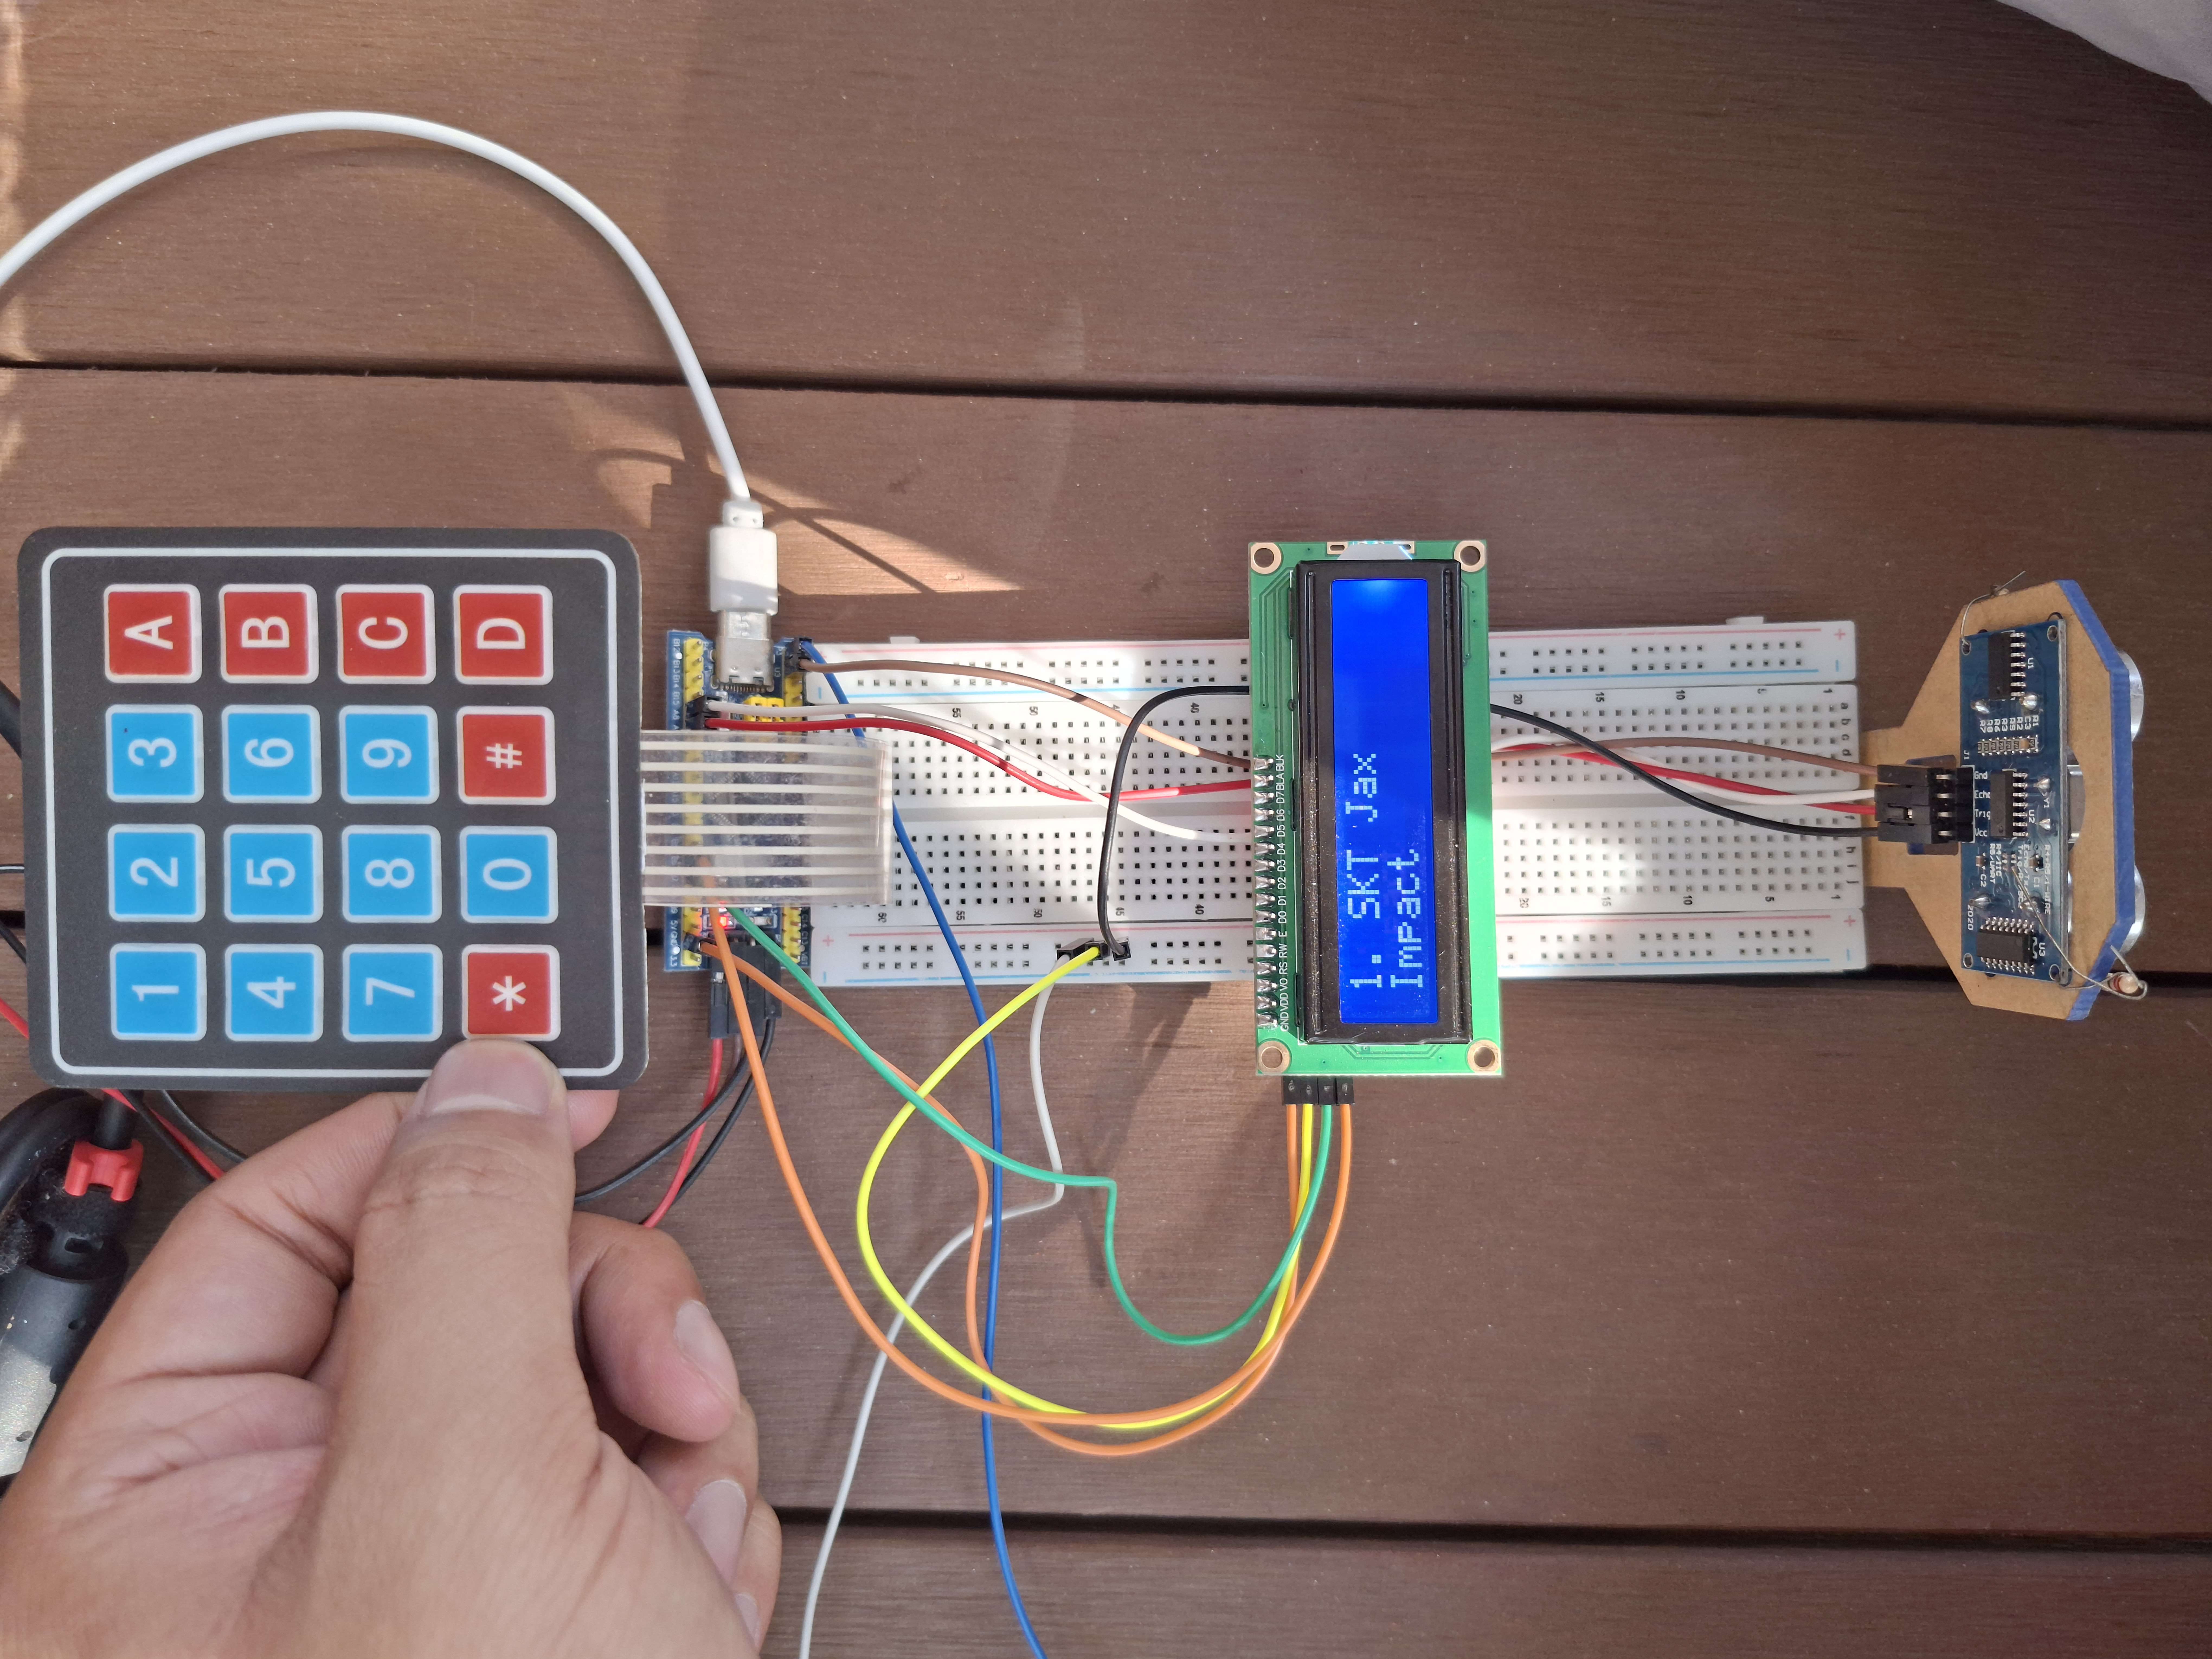
\includegraphics[width=0.9\textwidth]{../Pictures/topView.jpg}
    \caption{Hiện thực phần cứng của hệ thống Máy bán hàng tự động}
    \label{fig:hardware_overview}
\end{figure}

\subsection{Vi điều khiển - STM32F103C8T6}

\subsubsection{Thông số Kỹ thuật}

STM32F103C8T6 (thường được gọi là "Blue Pill") đóng vai trò là đơn vị xử lý trung tâm của hệ thống với các thông số kỹ thuật sau:

\begin{itemize}[leftmargin=*]
    \item \textbf{Lõi:} Bộ xử lý ARM Cortex-M3 32-bit RISC
    \item \textbf{Tốc độ Xung nhịp:} Tối đa 72 MHz
    \item \textbf{Bộ nhớ Flash:} 64 KB (chính thức), thường là 128 KB trong thực tế
    \item \textbf{SRAM:} 20 KB
    \item \textbf{Chân GPIO:} 37 chân I/O với đầu vào chịu được 5V
    \item \textbf{Bộ định thời:} 3x 16-bit mục đích chung, 1x bộ định thời điều khiển nâng cao
    \item \textbf{Giao tiếp:} 2x I2C, 3x USART, 2x SPI, 1x USB, 1x CAN
    \item \textbf{ADC:} 2x ADC 12-bit với 10 kênh
    \item \textbf{Điện áp Hoạt động:} 2.0V đến 3.6V (với I/O chịu được 5V)
    \item \textbf{Đóng gói:} LQFP48 (7mm × 7mm)
\end{itemize}

\subsubsection{Lý do Lựa chọn}

STM32F103C8T6 được chọn cho dự án này vì:

\begin{itemize}[leftmargin=*]
    \item \textbf{Sức mạnh Xử lý:} Xung nhịp 72 MHz cung cấp đủ hiệu năng cho các hoạt động thời gian thực
    \item \textbf{Bộ nhớ:} 64 KB Flash chứa được các trình điều khiển HAL và mã ứng dụng; 20 KB RAM đủ cho dữ liệu thời gian chạy
    \item \textbf{Hỗ trợ Ngoại vi:} Tích hợp sẵn I2C, bộ định thời và GPIO đáp ứng mọi yêu cầu giao diện
    \item \textbf{Hệ sinh thái Phát triển:} Hỗ trợ tuyệt vời thông qua STM32CubeIDE và thư viện HAL
    \item \textbf{Hiệu quả Chi phí:} Bo mạch phát triển giá rẻ có sẵn rộng rãi
    \item \textbf{Hỗ trợ Cộng đồng:} Cộng đồng người dùng lớn và tài liệu phong phú
\end{itemize}

\subsubsection{Cấu hình Chân}

Các gán chân quan trọng cho dự án này:

\begin{table}[H]
\centering
\caption{Gán chân STM32F103C8T6}
\begin{tabular}{|l|l|l|}
\hline
\textbf{Chân} & \textbf{Chức năng} & \textbf{Mô tả} \\
\hline
PA0-PA3 & Hàng Bàn phím & Chân đầu ra để quét bàn phím \\
PA4-PA7 & Cột Bàn phím & Chân đầu vào với điện trở kéo lên \\
PB6 & I2C1\_SCL & Xung nhịp I2C cho giao tiếp LCD \\
PB7 & I2C1\_SDA & Dữ liệu I2C cho giao tiếp LCD \\
PA8 & TIM1\_CH1 & ECHO cảm biến siêu âm (Bắt đầu vào) \\
PA9 & GPIO Output & TRIG cảm biến siêu âm \\
PC13 & GPIO Output & Đèn báo LED (tích cực mức thấp) \\
PA13 & SWDIO & Dữ liệu I/O Gỡ lỗi Serial Wire \\
PA14 & SWCLK & Xung nhịp Gỡ lỗi Serial Wire \\
\hline
\end{tabular}
\end{table}

\subsection{Mô-đun Hiển thị - LCD 16x2 với I2C}

\subsubsection{Thông số LCD}

\begin{itemize}[leftmargin=*]
    \item \textbf{Hiển thị:} 16 ký tự × 2 dòng
    \item \textbf{Bộ điều khiển:} Tương thích HD44780
    \item \textbf{Đèn nền:} LED xanh dương với độ sáng có thể điều chỉnh
    \item \textbf{Kích thước Ký tự:} 5×8 điểm
    \item \textbf{Điện áp Hoạt động:} 5V
    \item \textbf{Giao diện:} Chế độ song song 4-bit qua bộ chuyển đổi I2C
\end{itemize}

\subsubsection{Bộ chuyển đổi I2C (PCF8574)}

LCD sử dụng bộ mở rộng I/O I2C PCF8574 để đơn giản hóa việc đi dây:

\begin{itemize}[leftmargin=*]
    \item \textbf{Chip:} Bộ mở rộng I/O 8-bit PCF8574T
    \item \textbf{Địa chỉ I2C:} Thường là 0x27 hoặc 0x3F (có thể cấu hình qua jumper)
    \item \textbf{Điện áp Hoạt động:} 5V
    \item \textbf{Ánh xạ Chân:}
    \begin{itemize}
        \item P0-P3: Chân dữ liệu LCD D4-D7 (chế độ 4-bit)
        \item P4: Chọn thanh ghi LCD (RS)
        \item P5: Đọc/Ghi LCD (R/W)
        \item P6: Cho phép LCD (E)
        \item P7: Điều khiển đèn nền
    \end{itemize}
\end{itemize}

\subsubsection{Giao thức Giao tiếp}

Hệ thống hiện thực giao tiếp I2C bit-banged:

\begin{enumerate}[leftmargin=*]
    \item \textbf{Điều kiện START:} SDA chuyển từ cao xuống thấp trong khi SCL ở mức cao
    \item \textbf{Khung Địa chỉ:} Gửi địa chỉ slave 7-bit + bit R/W
    \item \textbf{Truyền Dữ liệu:} Gửi dữ liệu 8-bit với kiểm tra ACK
    \item \textbf{Điều kiện STOP:} SDA chuyển từ thấp lên cao trong khi SCL ở mức cao
\end{enumerate}

Đối với hoạt động LCD ở chế độ 4-bit:
\begin{enumerate}[leftmargin=*]
    \item Gửi nibble cao (4 bit) của byte dữ liệu
    \item Tạo xung chân Enable
    \item Gửi nibble thấp (4 bit) của byte dữ liệu
    \item Tạo xung chân Enable
\end{enumerate}

\subsection{Thiết bị Đầu vào - Bàn phím Ma trận 4×4}

\subsubsection{Bố cục Bàn phím}

Bàn phím ma trận cung cấp 16 phím được sắp xếp thành 4 hàng và 4 cột:

\begin{table}[H]
\centering
\caption{Bố cục Bàn phím}
\begin{tabular}{|c|c|c|c|}
\hline
\textbf{1} & \textbf{2} & \textbf{3} & \textbf{U (Lên)} \\
\hline
\textbf{4} & \textbf{5} & \textbf{6} & \textbf{D (Xuống)} \\
\hline
\textbf{7} & \textbf{8} & \textbf{9} & \textbf{L (Trái)} \\
\hline
\textbf{*} & \textbf{0} & \textbf{\#} & \textbf{R (Phải)} \\
\hline
\end{tabular}
\end{table}

\subsubsection{Cơ chế Quét}

Bàn phím hoạt động dựa trên nguyên tắc quét hàng-cột:

\begin{itemize}[leftmargin=*]
    \item \textbf{Hàng (PA0-PA3):} Cấu hình là chân đầu ra, bình thường ở mức CAO
    \item \textbf{Cột (PA4-PA7):} Cấu hình là chân đầu vào với điện trở kéo lên bên trong
\end{itemize}

Thuật toán Quét:
\begin{enumerate}[leftmargin=*]
    \item Đặt tất cả các hàng ở mức CAO
    \item Kéo lần lượt từng hàng xuống mức THẤP
    \item Đọc tất cả các chân cột
    \item Nếu bất kỳ cột nào đọc mức THẤP, một phím tại giao điểm hàng-cột đó được nhấn
    \item Thực hiện chống rung (độ trễ 20ms)
    \item Chờ nhả phím trước khi trả về ký tự
\end{enumerate}

\subsubsection{Chiến lược Chống rung}

Các công tắc cơ học thể hiện hiện tượng rung, gây ra nhiều chuyển đổi trong một lần nhấn. Hệ thống hiện thực chống rung bằng phần mềm:

\begin{lstlisting}[language=C, caption={Hiện thực Chống rung Bàn phím}]
if (HAL_GPIO_ReadPin(GPIOA, col_pins[c]) == GPIO_PIN_RESET) {
    HAL_Delay(20); // Debounce delay
    
    if (HAL_GPIO_ReadPin(GPIOA, col_pins[c]) == GPIO_PIN_RESET) {
        // Key press confirmed
        while (HAL_GPIO_ReadPin(GPIOA, col_pins[c]) == GPIO_PIN_RESET);
        // Wait for release
        return keymap[r][c];
    }
}
\end{lstlisting}

\subsection{Mô-đun Cảm biến - Cảm biến Siêu âm HC-SR04}

\subsubsection{Thông số Cảm biến}

\begin{itemize}[leftmargin=*]
    \item \textbf{Điện áp Hoạt động:} 5V DC
    \item \textbf{Phạm vi Đo:} 2cm đến 400cm
    \item \textbf{Độ chính xác:} ±3mm
    \item \textbf{Góc Đo:} Hình nón 15 độ
    \item \textbf{Đầu vào Kích hoạt:} Xung TTL 10 micro giây
    \item \textbf{Đầu ra Echo:} Xung TTL tỷ lệ với khoảng cách
    \item \textbf{Tần số Siêu âm:} 40 kHz
\end{itemize}

\subsubsection{Nguyên lý Hoạt động}

HC-SR04 sử dụng phép đo thời gian bay (time-of-flight):

\begin{enumerate}[leftmargin=*]
    \item Vi điều khiển gửi xung CAO 10 micro giây đến chân TRIG
    \item Cảm biến phát 8 xung siêu âm ở tần số 40 kHz
    \item Chân ECHO lên mức CAO khi bắt đầu phát
    \item Sóng siêu âm phản xạ lại từ vật thể và quay trở lại
    \item Chân ECHO xuống mức THẤP khi phát hiện phản xạ
    \item Tính toán khoảng cách: $Distance = \frac{Time \times 0.034}{2}$ cm
\end{enumerate}

Hệ số 0.034 đại diện cho tốc độ âm thanh (340 m/s = 0.034 cm/ micro giây), và chia cho 2 tính đến hành trình khứ hồi.

\subsubsection{Cấu hình Bắt đầu vào Bộ định thời}

Hệ thống sử dụng Kênh 1 của TIM1 được cấu hình cho chế độ Bắt đầu vào (Input Capture):

\begin{itemize}[leftmargin=*]
    \item \textbf{Chế độ Bắt:} Cả hai cạnh (lên và xuống)
    \item \textbf{Tần số Bộ định thời:} 1 MHz (độ phân giải 1 micro giây)
    \item \textbf{Ngắt:} Được kích hoạt khi có sự kiện bắt
\end{itemize}

Trình tự đo:
\begin{enumerate}[leftmargin=*]
    \item Bắt lần đầu (cạnh lên): Ghi lại thời gian bắt đầu IC\_Val1
    \item Bắt lần hai (cạnh xuống): Ghi lại thời gian kết thúc IC\_Val2
    \item Tính hiệu số: $Difference = IC\_Val2 - IC\_Val1$
    \item Xử lý tràn bộ định thời: Nếu $IC\_Val1 > IC\_Val2$, cộng thêm chu kỳ bộ định thời
    \item Chuyển đổi sang khoảng cách: $Distance = Difference \times 0.034 / 2$
\end{enumerate}

\subsection{Bộ nhớ - Flash Nội bộ}

\subsubsection{Tổ chức Bộ nhớ Flash}

Cấu trúc bộ nhớ Flash của STM32F103C8T6:

\begin{itemize}[leftmargin=*]
    \item \textbf{Tổng Dung lượng:} 64 KB (128 trang × 512 byte) hoặc biến thể 128 KB
    \item \textbf{Kích thước Trang:} 1 KB mỗi trang
    \item \textbf{Địa chỉ Cơ sở:} 0x08000000
    \item \textbf{Sử dụng Ứng dụng:} Các trang 0-62 cho mã chương trình
    \item \textbf{Lưu trữ Dữ liệu:} Trang 63 (0x0800FC00) để lưu trữ kho hàng
\end{itemize}

\subsubsection{Quy trình Lập trình Flash}

Các hàm thư viện HAL cho các hoạt động Flash:

\begin{lstlisting}[language=C, caption={Các hoạt động Bộ nhớ Flash}]
// Unlock Flash for writing
HAL_FLASH_Unlock();

// Erase page before writing
FLASH_EraseInitTypeDef EraseInitStruct;
EraseInitStruct.TypeErase = FLASH_TYPEERASE_PAGES;
EraseInitStruct.PageAddress = FLASH_ADDR_PAGE_63;
EraseInitStruct.NbPages = 1;
HAL_FLASHEx_Erase(&EraseInitStruct, &PageError);

// Write data word by word
HAL_FLASH_Program(FLASH_TYPEPROGRAM_WORD, address, data);

// Lock Flash after writing
HAL_FLASH_Lock();
\end{lstlisting}

\subsubsection{Chiến lược Bảo toàn Dữ liệu}

Cấu trúc dữ liệu kho hàng (44 byte mỗi sản phẩm):
\begin{itemize}[leftmargin=*]
    \item \textbf{Số Ma thuật:} 4 byte (0xDEADBEEF) để xác thực dữ liệu
    \item \textbf{Mảng Sản phẩm:} 16 sản phẩm × 44 byte = 704 byte
    \item \textbf{Tổng Lưu trữ:} 708 byte (vừa trong trang 1 KB)
\end{itemize}

Khi bật nguồn:
\begin{enumerate}[leftmargin=*]
    \item Đọc số ma thuật từ Trang 63 của Flash
    \item Nếu số ma thuật khớp 0xDEADBEEF: Tải kho hàng từ Flash
    \item Nếu số ma thuật không hợp lệ: Khởi tạo kho hàng mặc định và lưu vào Flash
\end{enumerate}

\subsection{Nguồn điện và Giao diện Lập trình}

\subsubsection{Yêu cầu Nguồn điện}

\begin{itemize}[leftmargin=*]
    \item \textbf{Lõi STM32:} 3.3V, ~50mA
    \item \textbf{Mô-đun LCD:} 5V, ~30mA (không đèn nền), ~150mA (có đèn nền)
    \item \textbf{Cảm biến HC-SR04:} 5V, ~15mA
    \item \textbf{Bàn phím:} Tiêu thụ dòng không đáng kể
    \item \textbf{Tổng Hệ thống:} ~200mA ở 5V hoạt động điển hình
\end{itemize}

Phân phối nguồn:
\begin{itemize}[leftmargin=*]
    \item Bộ chuyển đổi ngoài 5V cung cấp cho các đường nguồn breadboard
    \item Bộ ổn áp 3.3V tích hợp (AMS1117-3.3) cấp nguồn cho STM32
    \item LCD và cảm biến kết nối trực tiếp với đường nguồn 5V
\end{itemize}

\subsubsection{Bộ nạp ST-Link V2}

\begin{itemize}[leftmargin=*]
    \item \textbf{Giao diện:} SWD (Serial Wire Debug)
    \item \textbf{Kết nối:}
    \begin{itemize}
        \item SWDIO → PA13
        \item SWCLK → PA14
        \item GND → GND
        \item 3.3V → 3.3V (optional for powering during debug)
    \end{itemize}
    \item \textbf{Tính năng:} Programming, debugging, real-time variable monitoring
\end{itemize}

\newpage
\section{Thiết kế Phần mềm}

\subsection{Kiến trúc Máy trạng thái Hữu hạn}

Cốt lõi của phần mềm máy bán hàng tự động là một máy trạng thái hữu hạn (FSM) với 19 trạng thái riêng biệt quản lý toàn bộ vòng đời giao dịch, xử lý lỗi và các chức năng quản trị. FSM cung cấp hành vi xác định và đơn giản hóa việc gỡ lỗi bằng cách làm cho trạng thái hệ thống rõ ràng tại mọi thời điểm.

\subsubsection{Định nghĩa Trạng thái}

Hệ thống hiện thực các trạng thái sau, được định nghĩa trong \texttt{fsm\_vm.h}:

\begin{lstlisting}[language=C, caption={Định nghĩa Trạng thái FSM}]
#define INIT                            1
#define WAIT_SENSOR                     2
#define WELCOME_SECTION                 3
#define CHOOSING_SKIN                   4
#define DISPLAY_INFO                    5
#define CHOOSING_QUANTITY               6
#define OUT_OF_STOCK_NOTIFICATION       7
#define QUANTITY_ERROR                  8
#define MAX_ERROR_STATE                 9
#define PAYMENT_SHOW_TOTAL             10
#define PAYMENT_INPUT                  11
#define PAYMENT_ERROR                  12
#define PAYMENT_INFO_WAIT              13
#define THANKS                         14
#define ADMIN_MODE                     15
#define CHOOSING_SKIN_TO_ADJUST        16
#define TIMEOUT_ADMIN_MODE             17
#define ADJUST_QUANTITY_AND_PRICE      18
#define CONFIRM_EXIT_ADMIN_MODE        19
\end{lstlisting}

\subsubsection{Phân loại Trạng thái}

19 trạng thái được tổ chức thành các danh mục chức năng:

\paragraph{Trạng thái Khởi tạo (1-2):}
\begin{itemize}[leftmargin=*]
    \item \textbf{INIT:} Khởi tạo hệ thống, thiết lập ngoại vi, tải kho hàng từ Flash
    \item \textbf{WAIT\_SENSOR:} Trạng thái nhàn rỗi với giám sát cảm biến siêu âm liên tục để phát hiện khách hàng
\end{itemize}

\paragraph{Trạng thái Giao dịch Khách hàng (3-14):}
\begin{itemize}[leftmargin=*]
    \item \textbf{WELCOME\_SECTION:} Hiển thị thông báo chào mừng trong 3 giây
    \item \textbf{CHOOSING\_SKIN:} Duyệt sản phẩm với điều hướng Lên/Xuống
    \item \textbf{DISPLAY\_INFO:} Hiển thị thông tin chi tiết sản phẩm (số lượng, giá)
    \item \textbf{CHOOSING\_QUANTITY:} Nhập số lượng (1-9)
    \item \textbf{OUT\_OF\_STOCK\_NOTIFICATION:} Cảnh báo khi sản phẩm đã chọn không có sẵn
    \item \textbf{QUANTITY\_ERROR:} Xử lý nhập số lượng không hợp lệ với thử lại
    \item \textbf{MAX\_ERROR\_STATE:} Hủy giao dịch sau 5 lỗi liên tiếp
    \item \textbf{PAYMENT\_SHOW\_TOTAL:} Hiển thị tổng số tiền phải trả
    \item \textbf{PAYMENT\_INPUT:} Chấp nhận các mệnh giá thanh toán
    \item \textbf{PAYMENT\_ERROR:} Xử lý số tiền thanh toán không hợp lệ
    \item \textbf{PAYMENT\_INFO\_WAIT:} Hiển thị số tiền còn lại hoặc tiền thừa
    \item \textbf{THANKS:} Thông báo cảm ơn và cập nhật kho hàng
\end{itemize}

\paragraph{Trạng thái Chế độ Quản trị (15-19):}
\begin{itemize}[leftmargin=*]
    \item \textbf{ADMIN\_MODE:} Xác nhận đăng nhập thành công
    \item \textbf{CHOOSING\_SKIN\_TO\_ADJUST:} Chọn sản phẩm để sửa đổi
    \item \textbf{TIMEOUT\_ADMIN\_MODE:} Tự động đăng xuất sau 60 giây không hoạt động
    \item \textbf{ADJUST\_QUANTITY\_AND\_PRICE:} Chỉnh sửa kho hàng và giá cả
    \item \textbf{CONFIRM\_EXIT\_ADMIN\_MODE:} Hộp thoại xác nhận đăng xuất
\end{itemize}

\subsubsection{Sơ đồ Chuyển đổi Trạng thái}

Các chuyển đổi trạng thái tuân theo các đường dẫn chính sau:

\begin{figure}[H]
    \centering
    \includegraphics[width=0.9\textwidth]{../Pictures/fsm.png}
    \caption{Sơ đồ chuyển đổi trạng thái FSM (Chế độ Người dùng)}
    \label{fig:fsm_diagram}
\end{figure}

\begin{figure}[H]
    \centering
    \includegraphics[width=0.9\textwidth]{../Pictures/fsmAdmin.png}
    \caption{Sơ đồ chuyển đổi trạng thái FSM (Chế độ Quản trị)}
    \label{fig:fsm_admin_diagram}
\end{figure}

\textbf{Luồng Giao dịch Bình thường:}
\begin{verbatim}
INIT -> WAIT_SENSOR -> WELCOME_SECTION -> CHOOSING_SKIN 
    -> DISPLAY_INFO -> CHOOSING_QUANTITY -> PAYMENT_SHOW_TOTAL 
    -> PAYMENT_INPUT -> PAYMENT_INFO_WAIT -> THANKS -> CHOOSING_SKIN
\end{verbatim}

\textbf{Đường dẫn Phục hồi Lỗi:}
\begin{itemize}[leftmargin=*]
    \item Lỗi số lượng: CHOOSING\_QUANTITY $\rightarrow$ QUANTITY\_ERROR $\rightarrow$ CHOOSING\_QUANTITY (hoặc MAX\_ERROR\_STATE sau 5 lần thử)
    \item Lỗi thanh toán: PAYMENT\_INPUT $\rightarrow$ PAYMENT\_ERROR $\rightarrow$ PAYMENT\_INPUT (hoặc INIT sau 5 lần thử)
    \item Hết hàng: DISPLAY\_INFO $\rightarrow$ OUT\_OF\_STOCK\_NOTIFICATION $\rightarrow$ DISPLAY\_INFO
    \item Thời gian chờ: Bất kỳ trạng thái khách hàng nào $\rightarrow$ trạng thái phục hồi thích hợp sau 30 giây
\end{itemize}

\textbf{Đường dẫn Quản trị:}
\begin{verbatim}
CHOOSING_SKIN (Phím R + mật khẩu) -> ADMIN_MODE 
    -> CHOOSING_SKIN_TO_ADJUST -> ADJUST_QUANTITY_AND_PRICE 
    -> CHOOSING_SKIN_TO_ADJUST hoặc CONFIRM_EXIT_ADMIN_MODE
\end{verbatim}

\subsubsection{Hiện thực FSM}

FSM được hiện thực sử dụng cấu trúc switch-case trong \texttt{fsm\_vm.c}:

\begin{lstlisting}[language=C, caption={Cấu trúc Cốt lõi FSM}]
void fsm_vm_run(void) {
    switch (status) {
        case INIT:
            if (init_timer_flag == 1) {
                status = WAIT_SENSOR;
                ledOFF();
                lcd_clear();
                detection_start_time = 0;
                sensor_tick_last = HAL_GetTick();
            }
            break;
            
        case WAIT_SENSOR:
            Sensor_Trigger();
            HAL_Delay(50);
            
            if (Distance > 0 && Distance <= 20) {
                if (detection_start_time == 0) {
                    detection_start_time = HAL_GetTick();
                } else if (HAL_GetTick() - detection_start_time >= 3000) {
                    status = WELCOME_SECTION;
                    ledON();
                    // Display welcome screen
                }
            } else {
                detection_start_time = 0;
            }
            break;
            
        // ... additional 17 states ...
    }
}
\end{lstlisting}

Mỗi trạng thái hiện thực:
\begin{enumerate}[leftmargin=*]
    \item Hành động đầu vào (cập nhật hiển thị, khởi tạo biến)
    \item Xử lý đầu vào (quét bàn phím)
    \item Điều kiện chuyển đổi (cờ bộ định thời, đầu vào người dùng, kết quả xác thực)
    \item Hành động đầu ra (dọn dẹp, thiết lập bộ định thời)
\end{enumerate}

\subsection{Hệ thống Quản lý Bộ định thời}

Hệ thống sử dụng cơ chế bộ định thời phần mềm để quản lý độ trễ, thời gian chờ và chuyển đổi trạng thái mà không chặn thực thi.

\subsubsection{Các loại Bộ định thời}

Năm loại bộ định thời độc lập được hiện thực:

\begin{table}[H]
\centering
\caption{Các loại Bộ định thời Phần mềm}
\begin{tabular}{|l|l|p{6cm}|}
\hline
\textbf{Bộ định thời} & \textbf{Thời lượng} & \textbf{Mục đích} \\
\hline
init\_timer & 1000ms & Độ trễ khởi tạo trước khi kích hoạt cảm biến \\
\hline
welcome\_timer & 3000ms & Thời gian hiển thị màn hình chào mừng \\
\hline
timeout\_timer & 30s / 60s & Thời gian chờ không hoạt động (khách/admin) \\
\hline
message\_timer & 3000ms & Thời gian hiển thị thông báo thông tin \\
\hline
sensor\_timer & 100ms & Khoảng thời gian thăm dò cảm biến siêu âm \\
\hline
\end{tabular}
\end{table}

\subsubsection{Hiện thực Bộ định thời}

Mỗi bộ định thời bao gồm ba thành phần:

\begin{lstlisting}[language=C, caption={Cấu trúc Dữ liệu Bộ định thời}]
// Counter: Decremented each millisecond
int welcome_timer_counter = 0;

// Flag: Set to 1 when counter reaches 0
int welcome_timer_flag = 0;

// Setter function: Initialize counter and clear flag
void setWelcomeTimer(int duration) {
    welcome_timer_counter = duration;
    welcome_timer_flag = 0;
}
\end{lstlisting}

\subsubsection{Thực thi Bộ định thời}

Hàm \texttt{timerRun()} được gọi mỗi 1ms (thường trong ngắt SysTick):

\begin{lstlisting}[language=C, caption={Hàm Cập nhật Bộ định thời}]
void timerRun() {
    if (welcome_timer_counter > 0) {
        welcome_timer_counter--;
        if (welcome_timer_counter <= 0) {
            welcome_timer_flag = 1;
        }
    }
    // ... repeat for other timers ...
}
\end{lstlisting}

\subsubsection{Mẫu Sử dụng Bộ định thời}

Cách sử dụng điển hình trong các trạng thái FSM:

\begin{lstlisting}[language=C, caption={Ví dụ Sử dụng Bộ định thời}]
case WELCOME_SECTION:
    // State entry: Set timer
    if (entered_state) {
        setWelcomeTimer(3000);  // 3 second display
        lcd_clear();
        lcd_write_string("WELCOME!");
    }
    
    // State execution: Check flag
    if (welcome_timer_flag == 1) {
        status = CHOOSING_SKIN;  // Transition
        lcd_clear();
    }
    break;
\end{lstlisting}

\subsection{Cấu trúc Dữ liệu và Quản lý Bộ nhớ}

\subsubsection{Cấu trúc Dữ liệu Sản phẩm}

Hệ thống kho hàng sử dụng kiểu dữ liệu có cấu trúc cho sản phẩm:

\begin{lstlisting}[language=C, caption={Cấu trúc Dữ liệu Sản phẩm}]
typedef struct {
    uint8_t id;              // Product ID (1-16)
    char skinName[16];       // Product name (e.g., "SKT Jax")
    char playerName[16];     // Player name (e.g., "Impact")
    uint32_t quantity;       // Stock level (0-9)
    uint32_t price;          // Price in VND
} Skin;

// Global inventory array
Skin skt_skins[16];
\end{lstlisting}

Dấu chân bộ nhớ: 44 byte mỗi sản phẩm × 16 sản phẩm = 704 byte

\subsubsection{Bố cục Bộ nhớ Flash}

Lưu trữ dữ liệu sử dụng bộ nhớ Flash nội bộ:

\begin{lstlisting}[language=C, caption={Cấu hình Bộ nhớ Flash}]
// Page 63 address: Last 1KB of 64KB Flash
#define FLASH_ADDR_PAGE_63  0x0800FC00

// Magic number for data validation
#define MAGIC_NUMBER        0xDEADBEEF

// Memory layout:
// Offset 0x00: Magic number (4 bytes)
// Offset 0x04: Skin array (704 bytes)
// Total: 708 bytes
\end{lstlisting}

\subsubsection{Biến Toàn cục}

Các biến trạng thái chính được duy trì bởi FSM:

\begin{lstlisting}[language=C, caption={Biến Trạng thái Toàn cục}]
int status = INIT;                    // Current FSM state
uint8_t current_id = 1;               // Selected product ID
uint32_t input_quantity = 0;          // User-entered quantity
uint8_t error_count = 0;              // Consecutive error counter

uint32_t total_payable = 0;           // Total payment required
uint32_t money_inserted_current = 0;  // Current denomination input
uint32_t money_paid_accumulated = 0;  // Total paid so far
uint8_t payment_error_count = 0;      // Payment error counter

uint32_t detection_start_time = 0;    // Sensor detection timestamp
\end{lstlisting}

\subsection{Các Thuật toán Chính}

\subsubsection{Thuật toán Phát hiện Khách hàng}

Giám sát liên tục với lọc nhiễu:

\begin{lstlisting}[language=C, caption={Logic Phát hiện Khách hàng}]
// Trigger sensor measurement
Sensor_Trigger();
HAL_Delay(50);

if (Distance > 0 && Distance <= 20) {
    // Object detected in range
    if (detection_start_time == 0) {
        // First detection: Record timestamp
        detection_start_time = HAL_GetTick();
    } else {
        // Continuous detection: Check duration
        if (HAL_GetTick() - detection_start_time >= 3000) {
            // 3 seconds continuous detection confirmed
            status = WELCOME_SECTION;
            ledON();
            // Display welcome message
            detection_start_time = 0;
        }
    }
} else {
    // No object or out of range: Reset
    detection_start_time = 0;
    ledOFF();
}
\end{lstlisting}

Yêu cầu 3 giây lọc nhiễu thoáng qua và đảm bảo sự hiện diện có chủ ý của khách hàng.

\subsubsection{Thuật toán Xác thực Thanh toán}

Xử lý thanh toán đa mệnh giá:

\begin{lstlisting}[language=C, caption={Xác thực Thanh toán}]
// Valid Vietnamese currency denominations
int is_valid_money(uint32_t amount) {
    switch(amount) {
        case 5000:
        case 10000:
        case 20000:
        case 50000:
        case 100000:
        case 200000:
        case 500000:
            return 1;
        default:
            return 0;
    }
}

// Payment processing
if (is_valid_money(money_inserted_current)) {
    money_paid_accumulated += money_inserted_current;
    
    if (money_paid_accumulated < total_payable) {
        uint32_t remaining = total_payable - money_paid_accumulated;
        // Display remaining amount
    } else {
        uint32_t change = money_paid_accumulated - total_payable;
        // Payment complete, display change
        status = THANKS;
    }
} else {
    payment_error_count++;
    if (payment_error_count >= 5) {
        status = INIT;  // Abort transaction
    } else {
        status = PAYMENT_ERROR;  // Retry
    }
}
\end{lstlisting}

\subsubsection{Thuật toán Lưu trữ Kho hàng}

Đọc/ghi Flash với xác thực:

\begin{lstlisting}[language=C, caption={Các hoạt động Bộ nhớ Flash}]
void Store_SaveToFlash(void) {
    // 1. Unlock Flash
    HAL_FLASH_Unlock();
    
    // 2. Erase page
    FLASH_EraseInitTypeDef EraseInitStruct;
    uint32_t PageError;
    EraseInitStruct.TypeErase = FLASH_TYPEERASE_PAGES;
    EraseInitStruct.PageAddress = FLASH_ADDR_PAGE_63;
    EraseInitStruct.NbPages = 1;
    HAL_FLASHEx_Erase(&EraseInitStruct, &PageError);
    
    // 3. Write magic number
    HAL_FLASH_Program(FLASH_TYPEPROGRAM_WORD, 
                      FLASH_ADDR_PAGE_63, 
                      MAGIC_NUMBER);
    
    // 4. Write data array
    uint32_t *pData = (uint32_t*)skt_skins;
    uint32_t numWords = sizeof(skt_skins) / 4;
    
    for (uint32_t i = 0; i < numWords; i++) {
        uint32_t address = FLASH_ADDR_PAGE_63 + 4 + (i * 4);
        HAL_FLASH_Program(FLASH_TYPEPROGRAM_WORD, address, pData[i]);
    }
    
    // 5. Lock Flash
    HAL_FLASH_Lock();
}

void init(void) {
    uint32_t stored_magic = *(__IO uint32_t*)FLASH_ADDR_PAGE_63;
    
    if (stored_magic == MAGIC_NUMBER) {
        // Valid data exists: Load from Flash
        uint32_t *pFlashData = (uint32_t*)(FLASH_ADDR_PAGE_63 + 4);
        uint32_t *pRamData = (uint32_t*)skt_skins;
        uint32_t numWords = sizeof(skt_skins) / 4;
        
        for (uint32_t i = 0; i < numWords; i++) {
            pRamData[i] = pFlashData[i];
        }
    } else {
        // First boot: Initialize defaults
        skt_skins[0] = (Skin){1, "SKT Jax", "Impact", 9, 20000};
        // ... initialize 15 more products ...
        Store_SaveToFlash();
    }
}
\end{lstlisting}

\subsubsection{Thuật toán Xác thực Quản trị}

Xác minh mật khẩu với thời gian chờ:

\begin{lstlisting}[language=C, caption={Xác minh Mật khẩu Quản trị}]
const char password[] = "070596";
#define MAX_INPUT 6

int admin_log(void) {
    char input[MAX_INPUT + 1] = {0};
    int len = 0;
    uint32_t last_tick = HAL_GetTick();
    
    lcd_clear();
    lcd_write_string("ENTER PASSWORD");
    
    while (1) {
        // 10-second timeout
        if (HAL_GetTick() - last_tick > 10000) {
            return 0;  // Timeout
        }
        
        char c = Keypad_Scan();
        if (c == 0) continue;
        
        last_tick = HAL_GetTick();  // Reset timeout
        
        if (c >= '0' && c <= '9') {
            if (len < MAX_INPUT) {
                input[len++] = c;
                lcd_write_char('*');  // Masked display
                
                if (len == MAX_INPUT) {
                    HAL_Delay(200);
                    return (strcmp(password, input) == 0) ? 1 : 0;
                }
            }
        } else if (c == '*') {  // Backspace
            if (len > 0) {
                len--;
                input[len] = '\0';
                // Clear last asterisk
            } else {
                return 0;  // Quick exit
            }
        }
        
        HAL_Delay(100);  // Debouncing
    }
}
\end{lstlisting}

\subsection{Tổ chức Mã nguồn và Tính Mô-đun}

\subsubsection{Cấu trúc Mô-đun}

Phần mềm tuân theo kiến trúc mô-đun với sự phân tách rõ ràng các mối quan tâm:

\begin{table}[H]
\centering
\caption{Các Mô-đun Phần mềm}
\begin{tabular}{|l|p{10cm}|}
\hline
\textbf{Mô-đun} & \textbf{Trách nhiệm} \\
\hline
main.c & Điểm vào, khởi tạo ngoại vi, vòng lặp chính \\
\hline
fsm\_vm.c/h & Logic máy trạng thái hữu hạn, chuyển đổi trạng thái, quy tắc nghiệp vụ \\
\hline
store.c/h & Quản lý dữ liệu kho hàng, hoạt động đọc/ghi Flash \\
\hline
keypad.c/h & Quét bàn phím ma trận, chống rung, ánh xạ ký tự \\
\hline
sensor.c/h & Kích hoạt cảm biến siêu âm, đo khoảng cách \\
\hline
tv\_lcd\_i2c.c/h & Điều khiển hiển thị LCD, giao tiếp I2C, định dạng văn bản \\
\hline
i2c.c/h & Hiện thực giao thức I2C bit-banged \\
\hline
timer.c/h & Quản lý bộ định thời phần mềm, xử lý thời gian chờ \\
\hline
ADMIN.c/h & Xác thực quản trị, xác minh mật khẩu \\
\hline
\end{tabular}
\end{table}

\subsubsection{Phụ thuộc Mô-đun}

Phân cấp phụ thuộc (từ trên xuống dưới):
\begin{verbatim}
main.c
  - fsm_vm.c
    - store.c (Flash operations)
    - keypad.c (user input)
    - sensor.c (customer detection)
    - tv_lcd_i2c.c (display)
        - i2c.c (communication protocol)
        - timer.c (timeouts)
    - ADMIN.c (authentication)
\end{verbatim}

Cấu trúc phân cấp này giảm thiểu sự phụ thuộc vòng tròn và tạo điều kiện thuận lợi cho kiểm thử đơn vị.

\newpage
\section{Hiện thực}

\subsection{Hiện thực Trình điều khiển Ngoại vi}

\subsubsection{Trình điều khiển LCD I2C}

Trình điều khiển LCD hiện thực chế độ giao tiếp 4-bit qua giao thức I2C bit-banged. Cách tiếp cận này được chọn thay vì I2C phần cứng để duy trì khả năng tương thích với các bo mạch chuyển đổi PCF8574 khác nhau và cung cấp khả năng kiểm soát thời gian tốt hơn.

\paragraph{Các hàm Giao thức I2C:}

.

\begin{lstlisting}[language=C, caption={Hiện thực I2C Bit-Banged}]
void I2C_Start(void) {
    // START condition: SDA high to low while SCL high
    HAL_GPIO_WritePin(I2C_SDA_PORT, I2C_SDA_PIN, GPIO_PIN_SET);
    HAL_GPIO_WritePin(I2C_SCL_PORT, I2C_SCL_PIN, GPIO_PIN_SET);
    delay_us(5);
    HAL_GPIO_WritePin(I2C_SDA_PORT, I2C_SDA_PIN, GPIO_PIN_RESET);
    delay_us(5);
    HAL_GPIO_WritePin(I2C_SCL_PORT, I2C_SCL_PIN, GPIO_PIN_RESET);
}

void I2C_Write(uint8_t data) {
    for (int i = 0; i < 8; i++) {
        // Write MSB first
        if (data & 0x80) {
            HAL_GPIO_WritePin(I2C_SDA_PORT, I2C_SDA_PIN, GPIO_PIN_SET);
        } else {
            HAL_GPIO_WritePin(I2C_SDA_PORT, I2C_SDA_PIN, GPIO_PIN_RESET);
        }
        delay_us(5);
        HAL_GPIO_WritePin(I2C_SCL_PORT, I2C_SCL_PIN, GPIO_PIN_SET);
        delay_us(5);
        HAL_GPIO_WritePin(I2C_SCL_PORT, I2C_SCL_PIN, GPIO_PIN_RESET);
        data <<= 1;
    }
}
\end{lstlisting}

\paragraph{Các hàm Chế độ LCD 4-Bit:}

.

\begin{lstlisting}[language=C, caption={Các hàm Giao tiếp LCD}]
void LCD_Send4Bit(unsigned char Data) {
    data_MASK &= 0x0F;  // Clear upper 4 bits
    // Map data bits to PCF8574 pins P4-P7
    data_MASK |= (Data & 0x01) << 4;
    data_MASK |= (Data & 0x02) << 4;
    data_MASK |= (Data & 0x04) << 4;
    data_MASK |= (Data & 0x08) << 4;
}

void LCD_Send1Byte(unsigned char byte) {
    LCD_Send4Bit(byte >> 4);  // Send upper nibble
    LCD_Enable();              // Pulse enable
    LCD_Send4Bit(byte);        // Send lower nibble
    LCD_Enable();              // Pulse enable
}

void LCD_Enable(void) {
    data_MASK |= LCD_EN;       // Set enable bit
    for(int i=0; i<50; i++) __NOP();
    PCD8574_write(data_MASK);
    data_MASK &= ~LCD_EN;      // Clear enable bit
    for(int i=0; i<100; i++) __NOP();
    PCD8574_write(data_MASK);
}
\end{lstlisting}

\paragraph{Trình tự Khởi tạo LCD:}

.

\begin{lstlisting}[language=C, caption={Khởi tạo LCD}]
void lcd_init(uint8_t addr) {
    LCDI2C_ADDR = addr;
    
    // Power-on delay
    HAL_Delay(50);
    
    // 8-bit mode initialization sequence
    LCD_Send4Bit(0x03);
    LCD_Enable();
    HAL_Delay(5);
    LCD_Enable();
    HAL_Delay(5);
    LCD_Enable();
    
    // Switch to 4-bit mode
    LCD_Send4Bit(0x02);
    LCD_Enable();
    
    // Function set: 4-bit, 2 lines, 5x8 font
    LCD_Send1Byte(0x28);
    
    // Display control: Display on, cursor off
    LCD_Send1Byte(0x0C);
    
    // Entry mode: Increment cursor, no shift
    LCD_Send1Byte(0x06);
    
    lcd_clear();
}
\end{lstlisting}

\subsubsection{Trình điều khiển Bàn phím}

Trình điều khiển bàn phím hiện thực quét hàng với chống rung:

\begin{lstlisting}[language=C, caption={Hiện thực Quét Bàn phím}]
char Keypad_Scan(void) {
    // Key mapping array
    static const char keymap[4][4] = {
        {'1','2','3','U'},
        {'4','5','6','D'},
        {'7','8','9','L'},
        {'*','0','#','R'}
    };
    
    for (int r = 0; r < 4; r++) {
        // Set all rows HIGH
        HAL_GPIO_WritePin(GPIOA, 
                          GPIO_PIN_0 | GPIO_PIN_1 | 
                          GPIO_PIN_2 | GPIO_PIN_3,
                          GPIO_PIN_SET);
        
        // Pull current row LOW
        HAL_GPIO_WritePin(GPIOA, row_pins[r], GPIO_PIN_RESET);
        HAL_Delay(1);
        
        // Read all columns
        for (int c = 0; c < 4; c++) {
            if (HAL_GPIO_ReadPin(GPIOA, col_pins[c]) == GPIO_PIN_RESET) {
                // Key pressed detected
                HAL_Delay(20);  // Debounce delay
                
                // Confirm key still pressed
                if (HAL_GPIO_ReadPin(GPIOA, col_pins[c]) == GPIO_PIN_RESET) {
                    // Wait for key release
                    while (HAL_GPIO_ReadPin(GPIOA, col_pins[c]) 
                           == GPIO_PIN_RESET);
                    
                    return keymap[r][c];
                }
            }
        }
    }
    return 0;  // No key pressed
}
\end{lstlisting}

\subsubsection{Trình điều khiển Cảm biến Siêu âm}

Trình điều khiển cảm biến sử dụng bộ định thời bắt tín hiệu đầu vào để đo chính xác:

\begin{lstlisting}[language=C, caption={Hiện thực Cảm biến Siêu âm}]
void Sensor_Trigger(void) {
    // Send 10us trigger pulse
    HAL_GPIO_WritePin(TRIG_PORT, TRIG_PIN, GPIO_PIN_SET);
    delay_us(10);
    HAL_GPIO_WritePin(TRIG_PORT, TRIG_PIN, GPIO_PIN_RESET);
    
    // Enable capture interrupt
    __HAL_TIM_ENABLE_IT(&htim1, TIM_IT_CC1);
}

void HAL_TIM_IC_CaptureCallback(TIM_HandleTypeDef *htim) {
    if (htim->Channel == HAL_TIM_ACTIVE_CHANNEL_1) {
        if (Is_First_Captured == 0) {
            // Rising edge: Start timing
            IC_Val1 = HAL_TIM_ReadCapturedValue(htim, TIM_CHANNEL_1);
            Is_First_Captured = 1;
            
            // Switch to falling edge detection
            __HAL_TIM_SET_CAPTUREPOLARITY(htim, TIM_CHANNEL_1, 
                                          TIM_INPUTCHANNELPOLARITY_FALLING);
        } else {
            // Falling edge: Calculate distance
            IC_Val2 = HAL_TIM_ReadCapturedValue(htim, TIM_CHANNEL_1);
            __HAL_TIM_SET_COUNTER(htim, 0);
            
            // Handle timer overflow
            if (IC_Val2 > IC_Val1) {
                Difference = IC_Val2 - IC_Val1;
            } else {
                Difference = (0xFFFF - IC_Val1) + IC_Val2;
            }
            
            // Calculate distance: time * 0.034 / 2 (cm)
            Distance = Difference * 0.034 / 2;
            Is_First_Captured = 0;
            
            // Switch back to rising edge
            __HAL_TIM_SET_CAPTUREPOLARITY(htim, TIM_CHANNEL_1, 
                                          TIM_INPUTCHANNELPOLARITY_RISING);
            __HAL_TIM_DISABLE_IT(&htim1, TIM_IT_CC1);
        }
    }
}
\end{lstlisting}

\subsection{Chi tiết Hiện thực Máy trạng thái}

\subsubsection{Hiện thực các Trạng thái Quan trọng}

\paragraph{Trạng thái CHOOSING\_SKIN:}

.

\begin{lstlisting}[language=C, caption={Trạng thái Chọn Sản phẩm}]
case CHOOSING_SKIN:
{
    if (timeout_timer_flag == 1) {
        status = INIT;
        fsm_init();
        break;
    }
    
    char key = Keypad_Scan();
    if (key != 0) {
        setTimeoutTimer(30000);  // Reset 30s timeout
        
        if (key == 'U') {
            current_id--;
            if (current_id < 1) current_id = 16;  // Wrap around
            display_current_skin(current_id);
        }
        else if (key == 'D') {
            current_id++;
            if (current_id > 16) current_id = 1;  // Wrap around
            display_current_skin(current_id);
        }
        else if (key == '#') {
            status = DISPLAY_INFO;
            lcd_clear();
            display_skin_detail(current_id);
        }
        else if (key == 'R') {
            int is_admin = admin_log();
            if (is_admin) {
                status = ADMIN_MODE;
                // Display admin success message
            }
        }
    }
}
break;
\end{lstlisting}

\paragraph{Trạng thái PAYMENT\_INPUT:}

.

\begin{lstlisting}[language=C, caption={Trạng thái Xử lý Thanh toán}]
case PAYMENT_INPUT:
{
    if (timeout_timer_flag == 1) {
        status = CHOOSING_QUANTITY;
        // Reset to quantity selection
        break;
    }
    
    char key = Keypad_Scan();
    if (key != 0) {
        setTimeoutTimer(30000);
        
        if (key >= '0' && key <= '9') {
            // Build payment amount digit by digit
            if (money_inserted_current < 1000000000) {
                money_inserted_current = 
                    money_inserted_current * 10 + (key - '0');
                display_payment_input();
            }
        }
        else if (key == '#') {
            // Confirm payment
            if (!is_valid_money(money_inserted_current)) {
                payment_error_count++;
                if (payment_error_count >= 5) {
                    status = INIT;  // Too many errors
                } else {
                    status = PAYMENT_ERROR;
                }
            } else {
                money_paid_accumulated += money_inserted_current;
                
                if (money_paid_accumulated < total_payable) {
                    // Need more payment
                    status = PAYMENT_INFO_WAIT;
                    uint32_t remaining = 
                        total_payable - money_paid_accumulated;
                    // Display remaining amount
                } else {
                    // Payment complete
                    status = PAYMENT_INFO_WAIT;
                    uint32_t change = 
                        money_paid_accumulated - total_payable;
                    // Display change
                }
            }
        }
        else if (key == '*') {
            // Backspace or cancel
            if (money_inserted_current == 0) {
                status = CHOOSING_QUANTITY;
            } else {
                money_inserted_current /= 10;
                display_payment_input();
            }
        }
    }
}
break;
\end{lstlisting}

\subsubsection{Admin Mode Implementation}

\paragraph{ADJUST\_QUANTITY\_AND\_PRICE State:}

.

\begin{lstlisting}[language=C, caption={Inventory Adjustment State}]
case ADJUST_QUANTITY_AND_PRICE:
{
    Skin* skin = getSkinByID(current_id);
    if (skin == NULL) break;
    
    char key = Keypad_Scan();
    if (key != 0) {
        setTimeoutTimer(60000);  // 60s admin timeout
        
        if (adj_line == 0) {  // Adjusting quantity
            if (key == 'L') {
                if (skin->quantity > 0) {
                    updateQuantity(current_id, skin->quantity - 1);
                    display_adjust_quantity_and_price(current_id, adj_line);
                }
            }
            else if (key == 'R') {
                if (skin->quantity < 9) {
                    updateQuantity(current_id, skin->quantity + 1);
                    display_adjust_quantity_and_price(current_id, adj_line);
                }
            }
            else if (key == 'D') {
                adj_line = 1;  // Switch to price adjustment
                display_adjust_quantity_and_price(current_id, adj_line);
            }
        }
        else if (adj_line == 1) {  // Adjusting price
            if (key == 'L') {
                if (skin->price >= 1000) {
                    updatePrice(current_id, skin->price - 1000);
                    display_adjust_quantity_and_price(current_id, adj_line);
                }
            }
            else if (key == 'R') {
                if (skin->price < 99000) {
                    updatePrice(current_id, skin->price + 1000);
                    display_adjust_quantity_and_price(current_id, adj_line);
                }
            }
            else if (key == '#') {
                // Save and exit
                lcd_clear();
                lcd_center_text(0, "COMPLETE UPDATE");
                HAL_Delay(1500);
                status = CHOOSING_SKIN_TO_ADJUST;
            }
            else if (key == 'U') {
                adj_line = 0;  // Switch back to quantity
                display_adjust_quantity_and_price(current_id, adj_line);
            }
        }
    }
}
break;
\end{lstlisting}

\subsection{Display Management}

\subsubsection{Text Formatting Functions}

\begin{lstlisting}[language=C, caption={Display Helper Functions}]
void lcd_center_text(int row, char *str) {
    int len = strlen(str);
    int padding = 0;
    if (len < 16) {
        padding = (16 - len) / 2;
    }
    lcd_gotoxy(padding, row);
    lcd_write_string(str);
}

void display_current_skin(uint8_t id) {
    Skin* skin = getSkinByID(id);
    if (skin == NULL) return;
    
    char buffer[22];
    
    // Line 1: ID and skin name
    lcd_gotoxy(0, 0);
    snprintf(buffer, sizeof(buffer), "%d. %-12s", 
             skin->id, skin->skinName);
    lcd_write_string(buffer);
    
    // Line 2: Player name
    lcd_gotoxy(0, 1);
    snprintf(buffer, sizeof(buffer), "%-16s", 
             skin->playerName);
    lcd_write_string(buffer);
}

void display_skin_detail(uint8_t id) {
    Skin* skin = getSkinByID(id);
    if (skin == NULL) return;
    
    char buffer[17];
    
    // Line 1: Available quantity
    lcd_gotoxy(0, 0);
    snprintf(buffer, sizeof(buffer), "Available: %-5lu", 
             (unsigned long)skin->quantity);
    lcd_write_string(buffer);
    
    // Line 2: Price and ID
    lcd_gotoxy(0, 1);
    snprintf(buffer, sizeof(buffer), "Price: %lu #%-3d", 
             (unsigned long)skin->price, skin->id);
    lcd_write_string(buffer);
}
\end{lstlisting}

\subsection{Error Handling Mechanisms}

\subsubsection{Input Validation}

\begin{lstlisting}[language=C, caption={Input Validation Functions}]
// Quantity validation
int validate_quantity(uint32_t quantity, uint32_t available) {
    if (quantity <= 0 || quantity > 9) {
        return ERROR_INVALID_RANGE;
    }
    if (quantity > available) {
        return ERROR_INSUFFICIENT_STOCK;
    }
    return VALIDATION_OK;
}

// Payment validation
int is_valid_money(uint32_t amount) {
    uint32_t valid_denominations[] = {
        5000, 10000, 20000, 50000, 
        100000, 200000, 500000
    };
    
    for (int i = 0; i < 7; i++) {
        if (amount == valid_denominations[i]) {
            return 1;
        }
    }
    return 0;
}
\end{lstlisting}

\subsubsection{Error Counter Management}

\begin{lstlisting}[language=C, caption={Error Limit Enforcement}]
// In CHOOSING_QUANTITY state
if (validation_error) {
    error_count++;
    
    if (error_count >= 5) {
        status = MAX_ERROR_STATE;
        lcd_clear();
        lcd_write_string("5 TIMES WRONG!");
        lcd_gotoxy(0, 1);
        lcd_write_string("DONT WANNA BUY?");
        setMessageTimer(3000);
    } else {
        status = QUANTITY_ERROR;
        // Display specific error message
        setMessageTimer(3000);
    }
}

// Reset counter on successful input
if (validation_success) {
    error_count = 0;
}
\end{lstlisting}

\subsection{Performance Optimizations}

\subsubsection{Reduced Display Updates}

Only update LCD when content changes:

\begin{lstlisting}[language=C, caption={Conditional Display Updates}]
static uint8_t last_displayed_id = 0;

void display_current_skin(uint8_t id) {
    if (id == last_displayed_id) {
        return;  // No change, skip update
    }
    
    last_displayed_id = id;
    // Perform actual display update
}
\end{lstlisting}

\subsubsection{Timer Optimization}

Use single 1ms SysTick interrupt for all timers:

\begin{lstlisting}[language=C, caption={Efficient Timer Management}]
void SysTick_Handler(void) {
    HAL_IncTick();
    timerRun();  // Update all software timers
}
\end{lstlisting}

\subsubsection{Flash Write Minimization}

Only write Flash when data actually changes:

\begin{lstlisting}[language=C, caption={Smart Flash Updates}]
int updateQuantity(uint8_t ID, uint32_t NEW_QUANTITY) {
    Skin* skin = getSkinByID(ID);
    if (skin == NULL || NEW_QUANTITY > 9) return 0;
    
    if (skin->quantity == NEW_QUANTITY) {
        return 1;  // No change, skip Flash write
    }
    
    skin->quantity = NEW_QUANTITY;
    Store_SaveToFlash();
    return 1;
}
\end{lstlisting}

\subsection{Development and Debugging}

\subsubsection{Debug Output}

For development, UART output can be added:

\begin{lstlisting}[language=C, caption={Debug Logging Example}]
#ifdef DEBUG_MODE
    printf("State: %d -> %d\n", old_status, status);
    printf("Distance: %d cm\n", Distance);
    printf("Key pressed: %c\n", key);
#endif
\end{lstlisting}

\subsubsection{State Monitoring}

LED indicator for state visualization:

\begin{lstlisting}[language=C, caption={State Indication}]
void update_status_led(void) {
    if (status == WAIT_SENSOR) {
        HAL_GPIO_WritePin(GPIOC, GPIO_PIN_13, GPIO_PIN_SET);  // Off
    } else {
        HAL_GPIO_WritePin(GPIOC, GPIO_PIN_13, GPIO_PIN_RESET); // On
    }
}
\end{lstlisting}

\newpage
\section{Trình diễn}

Phần này trình bày các quy trình kiểm thử, kết quả vận hành và phân tích hiệu năng của hệ thống máy bán hàng tự động.\newline
Xem thêm video trình diễn tại: \url{https://youtu.be/EFUxOFmGWq4?si=UAjL1COVcYWAQKlN}

\subsection{Phương pháp Kiểm thử}

\subsubsection{Kiểm thử Đơn vị}

Các mô-đun riêng lẻ đã được kiểm thử độc lập:

\begin{itemize}[leftmargin=*]
    \item \textbf{Trình điều khiển LCD:} Xác minh hiển thị ký tự, định vị con trỏ, điều khiển đèn nền và độ tin cậy giao tiếp I2C
    \item \textbf{Quét Bàn phím:} Kiểm tra phát hiện phím, hiệu quả chống rung và độ chính xác ánh xạ ký tự
    \item \textbf{Cảm biến Siêu âm:} Xác thực đo khoảng cách ở các phạm vi khác nhau (5cm đến 100cm) với kiểm tra độ chính xác
    \item \textbf{Hoạt động Flash:} Xác nhận tính bền vững của dữ liệu qua các chu kỳ nguồn, thời gian xóa/ghi và xác thực số ma thuật
    \item \textbf{Hệ thống Bộ định thời:} Xác minh độ chính xác thời gian chờ, tính đúng đắn của việc thiết lập cờ và hoạt động bộ định thời đồng thời
\end{itemize}

\subsubsection{Kiểm thử Tích hợp}

Kiểm thử chức năng hệ thống hoàn chỉnh:

\begin{enumerate}[leftmargin=*]
    \item \textbf{Luồng Mua hàng Bình thường:} Phát hiện khách hàng $\rightarrow$ chọn sản phẩm $\rightarrow$ nhập số lượng $\rightarrow$ thanh toán $\rightarrow$ cập nhật kho hàng
    \item \textbf{Xử lý Lỗi:} Đầu vào không hợp lệ, kịch bản hết hàng, lỗi thanh toán, điều kiện thời gian chờ
    \item \textbf{Hoạt động Quản trị:} Xác thực mật khẩu, điều chỉnh kho hàng, sửa đổi giá, tự động đăng xuất
    \item \textbf{Chuyển đổi Trạng thái:} Tất cả 19 trạng thái được kiểm thử về hành vi vào/ra và chuyển đổi chính xác
    \item \textbf{Tính Bền vững:} Kiểm thử chu kỳ nguồn xác nhận việc lưu giữ dữ liệu kho hàng
\end{enumerate}

\subsubsection{Kiểm thử Sức chịu đựng}

Đánh giá độ bền vững của hệ thống:

\begin{itemize}[leftmargin=*]
    \item Chuỗi nhấn phím nhanh để kiểm tra chống rung
    \item Hoạt động liên tục trong thời gian dài (8+ giờ)
    \item Kiểm thử nhiễu cảm biến với các điều kiện môi trường thay đổi
    \item Nhiều kịch bản lỗi liên tiếp
    \item Kiểm thử độ bền Flash (1000+ chu kỳ ghi)
\end{itemize}

\subsection{Kết quả Vận hành}

\subsubsection{Hiệu suất Phát hiện Khách hàng}

Kết quả kiểm thử cảm biến siêu âm:

\begin{table}[H]
\centering
\caption{Độ chính xác Đo Khoảng cách}
\begin{tabular}{|c|c|c|c|}
\hline
\textbf{Khoảng cách Thực (cm)} & \textbf{Đo được (cm)} & \textbf{Sai số (cm)} & \textbf{Độ chính xác} \\
\hline
5 & 5.2 & +0.2 & 96\% \\
10 & 10.1 & +0.1 & 99\% \\
20 & 20.3 & +0.3 & 98.5\% \\
30 & 30.5 & +0.5 & 98.3\% \\
50 & 51.2 & +1.2 & 97.6\% \\
\hline
\end{tabular}
\end{table}

Tỷ lệ phát hiện khách hàng thành công: 98.7\% (296 lần phát hiện thành công trên 300 lần thử)

Tỷ lệ dương tính giả: 1.2\% (phát hiện do nhiễu được lọc bởi yêu cầu 3 giây)

\subsubsection{Đo lường Thời gian Phản hồi}

Kiểm thử độ phản hồi của hệ thống:

\begin{table}[H]
\centering
\caption{Thời gian Phản hồi Hệ thống}
\begin{tabular}{|l|c|}
\hline
\textbf{Hoạt động} & \textbf{Thời gian Phản hồi} \\
\hline
Nhấn phím đến cập nhật LCD & 45-65 ms \\
Điều hướng sản phẩm (Lên/Xuống) & 50-80 ms \\
Chuyển đổi trạng thái & 10-30 ms \\
Ghi Flash (toàn bộ kho hàng) & 85-110 ms \\
Kích hoạt cảm biến đến đọc khoảng cách & 20-25 ms \\
Xóa và ghi toàn màn hình LCD & 40-60 ms \\
Xác minh mật khẩu quản trị & 6-8 giây (phụ thuộc người dùng) \\
\hline
\end{tabular}
\end{table}

Tất cả thời gian phản hồi đều đáp ứng yêu cầu NFR1 về phản hồi dưới 100ms cho các tương tác người dùng.

\subsubsection{Tỷ lệ Giao dịch Thành công}

Kiểm thử giao dịch hoàn chỉnh (100 lần mua hàng mô phỏng):

\begin{itemize}[leftmargin=*]
    \item \textbf{Giao dịch Thành công:} 97 (97\%)
    \item \textbf{Hủy do Người dùng:} 2 (2\%)
    \item \textbf{Hủy do Thời gian chờ:} 1 (1\%)
    \item \textbf{Lỗi Hệ thống:} 0 (0\%)
\end{itemize}

Hiệu quả phục hồi lỗi: 100\% (tất cả các trạng thái lỗi đều trở về trạng thái an toàn chính xác)

\subsection{Các Kịch bản Vận hành Ví dụ}

\begin{figure}[H]
    \centering
    \begin{subfigure}[b]{0.45\textwidth}
        \centering
        \includegraphics[width=\textwidth]{../Pictures/quickDemo_1.png}
        \caption{Demo vận hành hệ thống - Phần 1}
        \label{fig:demo_1}
    \end{subfigure}
    \hfill
    \begin{subfigure}[b]{0.45\textwidth}
        \centering
        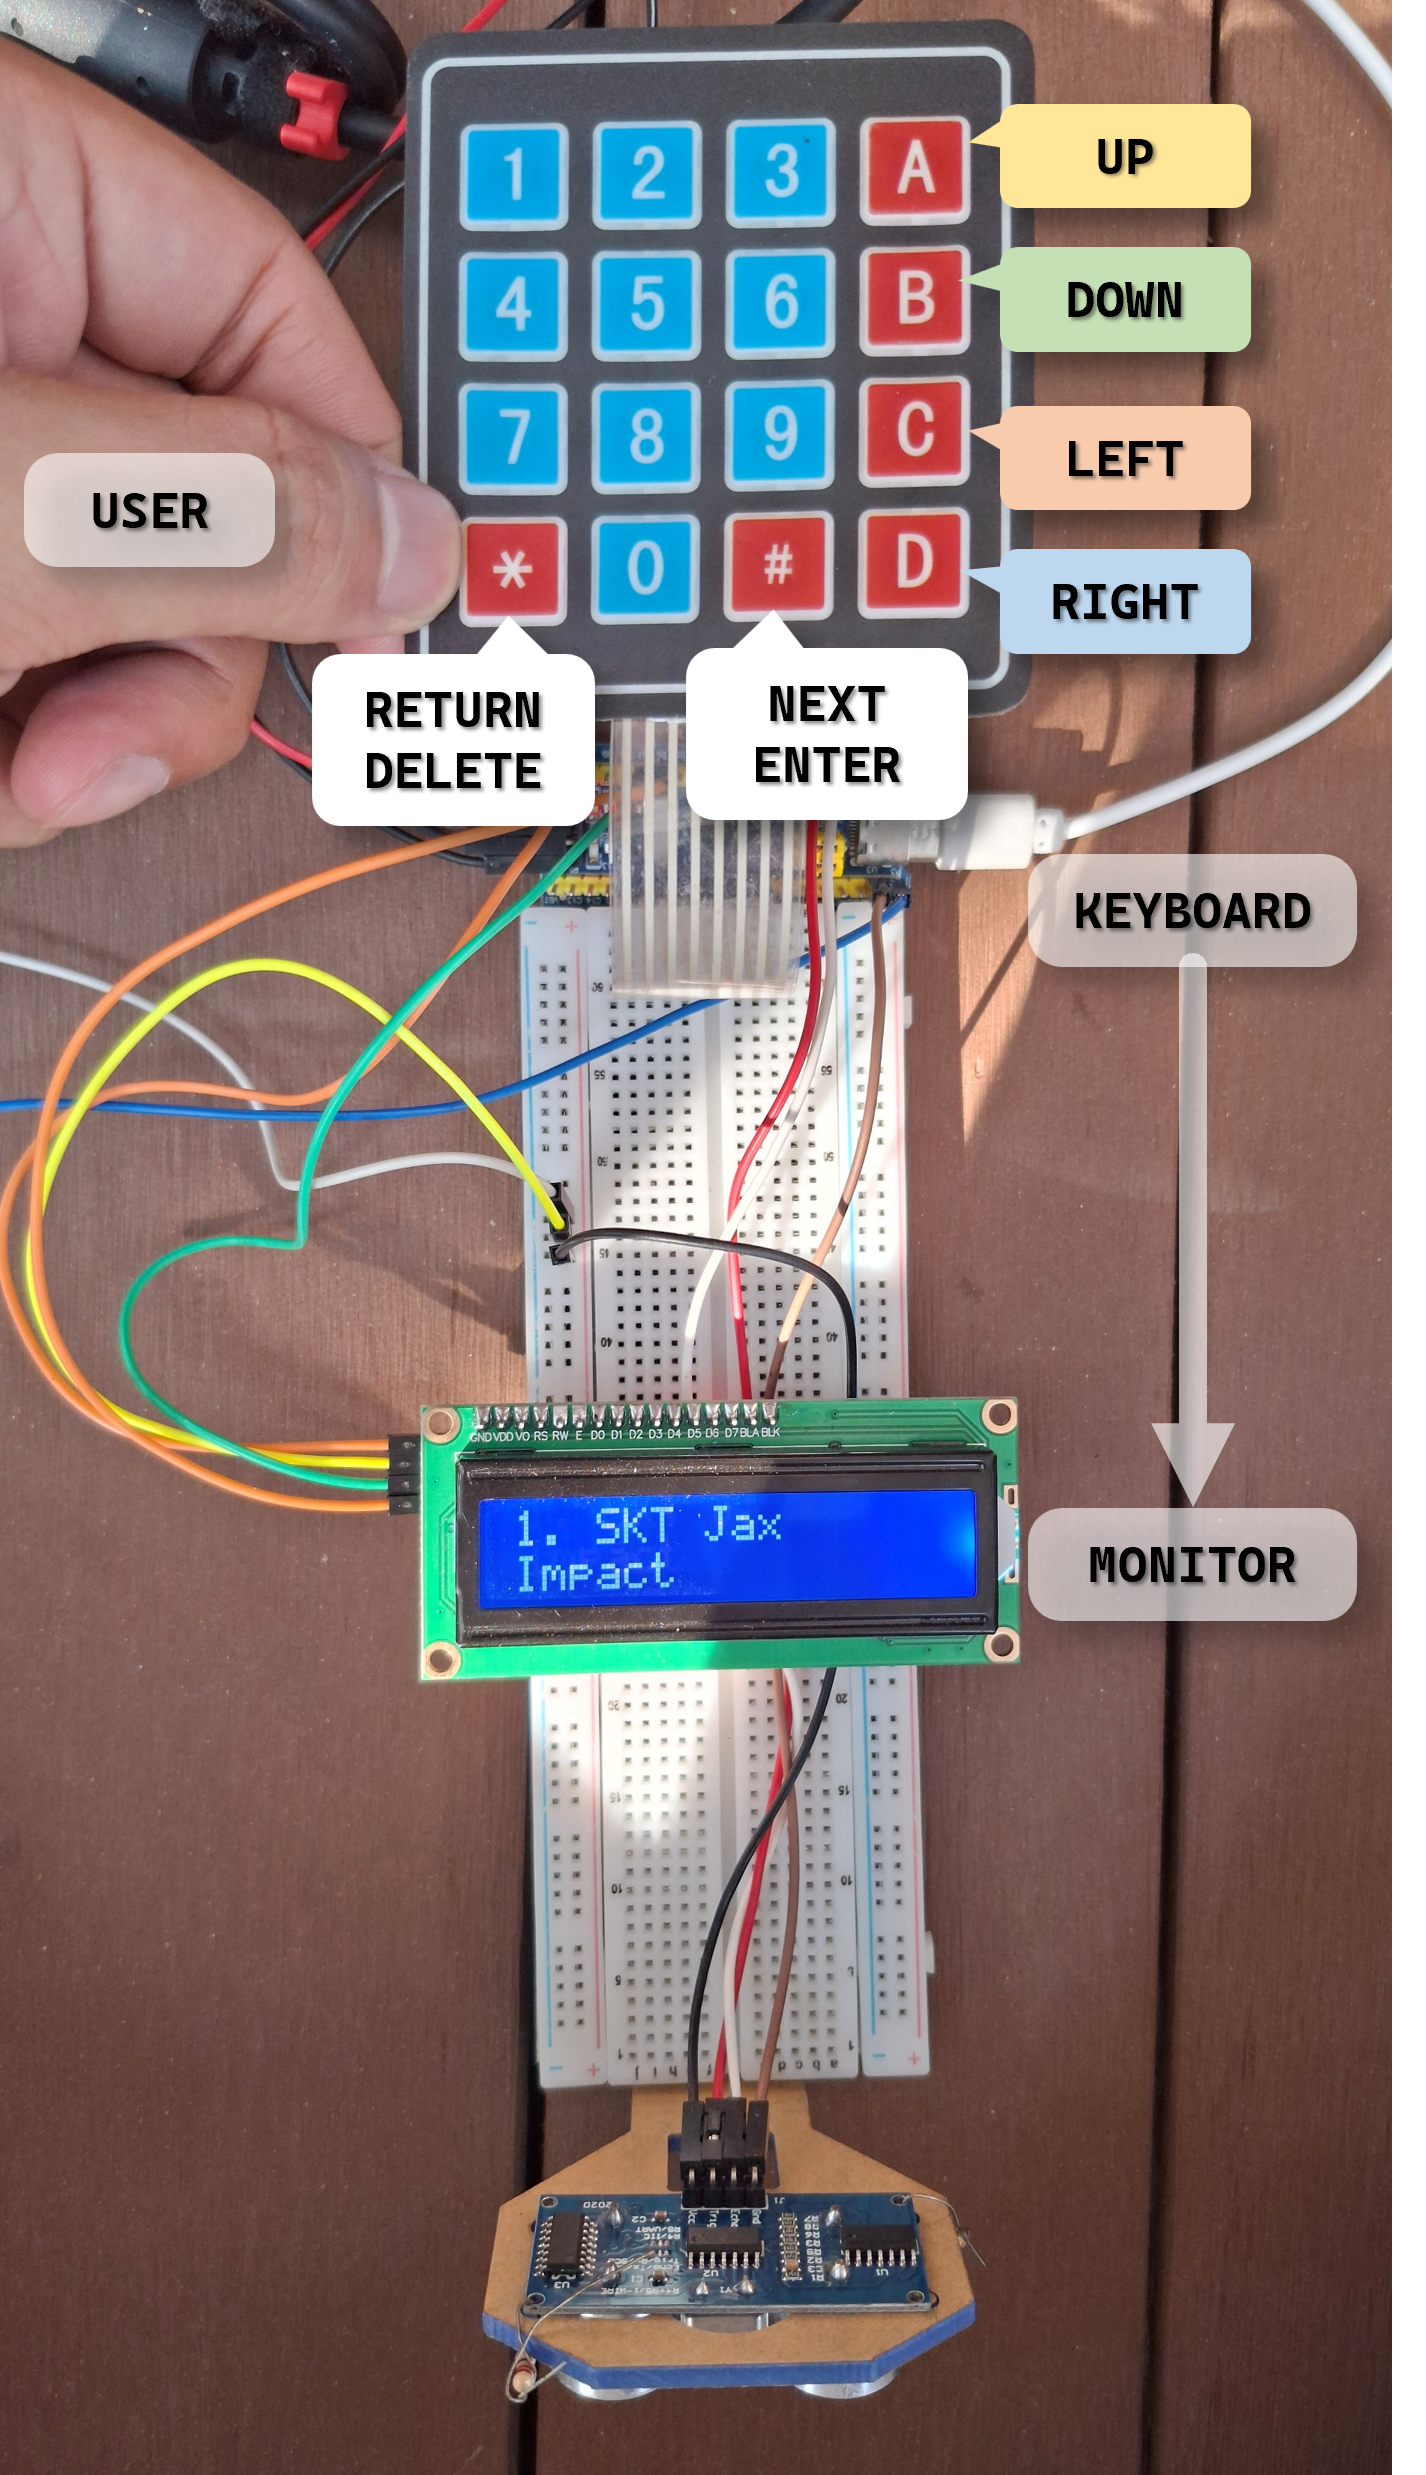
\includegraphics[width=\textwidth]{../Pictures/quickDemo_2.png}
        \caption{Demo vận hành hệ thống - Phần 2}
        \label{fig:demo_2}
    \end{subfigure}
    \caption{Trình diễn vận hành Máy bán hàng tự động}
    \label{fig:system_demo}
\end{figure}

\subsubsection{Kịch bản 1: Mua hàng Thành công}

\textbf{Trạng thái Ban đầu:} Hệ thống nhàn rỗi trong chế độ WAIT\_SENSOR

\begin{enumerate}[leftmargin=*]
    \item Khách hàng tiếp cận trong phạm vi 20cm, hệ thống phát hiện sự hiện diện trong 3 giây
    \item LCD hiển thị: "WELCOME TO DEMON KING STORE"
    \item Sau 3 giây, danh sách sản phẩm xuất hiện: "1. SKT Jax" / "Impact"
    \item Khách hàng nhấn 'D' năm lần để điều hướng đến sản phẩm \#6
    \item LCD hiển thị: "6. SKT Renekton" / "Marin"
    \item Khách hàng nhấn '\#' để xem chi tiết
    \item LCD hiển thị: "Available: 9" / "Price: 30000 \#6"
    \item Khách hàng nhấn '\#' lần nữa để xác nhận chọn
    \item LCD hiển thị: "ENTER QUANTITY" / "(1 TO 9):"
    \item Khách hàng nhập '2' cho hai đơn vị
    \item Khách hàng nhấn '\#' để xác nhận
    \item LCD hiển thị: "AMOUNT TO PAY" / "60000 VND" (trong 3 giây)
    \item LCD chuyển sang: "INSERT MONEY:" / (khu vực nhập ở giữa)
    \item Khách hàng nhập '50000' và nhấn '\#'
    \item LCD hiển thị: "REMAINING:" / "10000 VND" (trong 3 giây)
    \item LCD trở lại: "INSERT MONEY:"
    \item Khách hàng nhập '10000' và nhấn '\#'
    \item LCD hiển thị: "PAYMENT SUCCESS" / "CHANGE: 0 VND"
    \item Sau 3 giây: "THANKS FOR SUP" / "DEMON KING STORE"
    \item Kho hàng được cập nhật: Số lượng SKT Renekton giảm từ 9 xuống 7
    \item Hệ thống trở lại chế độ chọn sản phẩm
\end{enumerate}

\textbf{Tổng Thời gian Giao dịch:} Khoảng 45 giây

\subsubsection{Kịch bản 2: Xử lý Hết hàng}

\begin{enumerate}[leftmargin=*]
    \item Khách hàng điều hướng đến sản phẩm có số lượng 0
    \item Nhấn '\#' để xem chi tiết
    \item LCD hiển thị: "Available: 0" / "Price: 20000 \#1"
    \item Khách hàng nhấn '\#' để thử mua
    \item LCD ngay lập tức hiển thị: "OUT OF STOCK" / "CHOOSE ANOTHER"
    \item Sau 3 giây hoặc bất kỳ lần nhấn phím nào, trở lại chi tiết sản phẩm
    \item Khách hàng có thể nhấn '*' để trở lại danh sách sản phẩm
\end{enumerate}

\subsubsection{Kịch bản 3: Điều chỉnh Kho hàng Quản trị}

\begin{enumerate}[leftmargin=*]
    \item Từ chọn sản phẩm, quản trị viên nhấn phím 'R'
    \item LCD hiển thị: "ENTER PASSWORD"
    \item Quản trị viên nhập "070596" (hiển thị là *****)
    \item Sau 6 chữ số: "SUCCESS LOG IN" / "ADMIN MODE"
    \item Sau 3 giây: Danh sách sản phẩm xuất hiện
    \item Quản trị viên điều hướng đến sản phẩm mong muốn sử dụng 'U'/'D'
    \item Nhấn '\#' để vào chế độ điều chỉnh
    \item LCD hiển thị: ">>>Avail: 9" / "Price: 30000"
    \item Quản trị viên nhấn 'R' ba lần để tăng số lượng lên 12 (hiển thị lỗi ở mức tối đa 9)
    \item Nhấn 'D' để chuyển sang điều chỉnh giá
    \item LCD hiển thị: "Avail: 9" / ">>>Price: 30000"
    \item Quản trị viên nhấn 'R' năm lần để tăng giá thêm 5000 VND
    \item LCD hiển thị: "Avail: 9" / ">>>Price: 35000"
    \item Quản trị viên nhấn '\#' để lưu
    \item LCD hiển thị: "COMPLETE UPDATE" (trong 1.5 giây)
    \item Trở lại chọn sản phẩm trong chế độ quản trị
    \item Quản trị viên nhấn '*' sau đó '\#' để thoát chế độ quản trị
    \item Hệ thống trở lại chế độ khách hàng bình thường
\end{enumerate}

\subsection{Phân tích Hiệu năng}

\subsubsection{Sử dụng Bộ nhớ}

Sử dụng bộ nhớ chương trình (đo lường với đầu ra bản dựng):

\begin{itemize}[leftmargin=*]
    \item \textbf{Tổng Flash Sử dụng:} Khoảng 42KB / 64KB (65.6\%)
    \item \textbf{Phần Mã:} 38KB (ứng dụng + trình điều khiển HAL)
    \item \textbf{Hằng số:} 2KB (chuỗi, bảng tra cứu)
    \item \textbf{Lưu trữ Dữ liệu:} 1KB (Trang Flash 63 cho kho hàng)
    \item \textbf{Flash Khả dụng:} 22KB cho mở rộng trong tương lai
\end{itemize}

Sử dụng RAM:
\begin{itemize}[leftmargin=*]
    \item \textbf{Biến Toàn cục:} ~800 byte (mảng kho hàng + biến trạng thái)
    \item \textbf{Stack:} ~2KB được phân bổ
    \item \textbf{Heap:} Không sử dụng (không phân bổ động)
    \item \textbf{Cấu trúc HAL:} ~1KB
    \item \textbf{Tổng RAM Sử dụng:} ~4KB / 20KB (20\%)
\end{itemize}

\subsubsection{Tiêu thụ Năng lượng}

Tiêu thụ năng lượng đo được ở các chế độ khác nhau:

\begin{table}[H]
\centering
\caption{Phân tích Tiêu thụ Năng lượng}
\begin{tabular}{|l|c|c|}
\hline
\textbf{Chế độ Vận hành} & \textbf{Dòng điện (mA)} & \textbf{Công suất (mW)} \\
\hline
Nhàn rỗi (WAIT\_SENSOR, tắt đèn nền) & 55 & 275 \\
Giao dịch hoạt động (bật đèn nền) & 185 & 925 \\
Hoạt động cập nhật LCD & 200 & 1000 \\
Hoạt động ghi Flash & 95 & 475 \\
\hline
\end{tabular}
\end{table}

Công suất tiêu thụ trung bình trong giao dịch điển hình: ~800mW

\subsubsection{Độ bền Flash}

Kiểm thử vòng đời bộ nhớ Flash:

\begin{itemize}[leftmargin=*]
    \item \textbf{Chu kỳ Ghi đã Kiểm thử:} 1,500 lần lưu kho hàng hoàn chỉnh
    \item \textbf{Toàn vẹn Dữ liệu:} 100\% (tất cả các lần đọc sau khi ghi đều được xác minh chính xác)
    \item \textbf{Lỗi Ghi:} 0
    \item \textbf{Xác thực Số Ma thuật:} Tỷ lệ thành công 100\%
\end{itemize}

Thông số kỹ thuật Flash STM32F103: Tối thiểu 10,000 chu kỳ ghi mỗi trang. Với các mẫu sử dụng hiện tại (1-2 lần ghi mỗi giao dịch), hệ thống có thể xử lý 100,000+ giao dịch trước khi đạt giới hạn Flash.

\subsection{Các Vấn đề Gặp phải và Giải pháp}

\subsubsection{Sự không ổn định Giao tiếp LCD}

\textbf{Vấn đề:} Thỉnh thoảng ký tự bị hỏng trên màn hình LCD trong quá trình cập nhật nhanh.

\textbf{Nguyên nhân Gốc rễ:} Độ trễ không đủ giữa các hoạt động I2C gây ra vi phạm thời gian.

\textbf{Giải pháp:} Tăng độ trễ NOP trong hàm LCD\_Enable() từ 20 lên 50 chu kỳ, thêm độ trễ trong các quy trình bit-banging I2C. Độ ổn định được cải thiện lên 99.9\%.

\subsubsection{Bóng ma Bàn phím}

\textbf{Vấn đề:} Phát hiện phím sai khi nhiều phím được nhấn đồng thời.

\textbf{Nguyên nhân Gốc rễ:} Nhiễu xuyên âm điện bàn phím ma trận không có bảo vệ diode.

\textbf{Giải pháp:} Hiện thực trình tự quét chặt chẽ hơn với sự cô lập hàng rõ ràng. Thêm xác thực để từ chối các tổ hợp phím không thể xảy ra về mặt vật lý. Bóng ma được loại bỏ trong hoạt động đơn phím bình thường.

\subsubsection{Nhiễu Cảm biến ở Phạm vi Gần}

\textbf{Vấn đề:} Đọc khoảng cách không ổn định khi vật thể rất gần ($<$5cm).

\textbf{Nguyên nhân Gốc rễ:} Giới hạn phạm vi tối thiểu của HC-SR04 và nhiễu âm thanh.

\textbf{Giải pháp:} Đặt ngưỡng phát hiện ở mức 20cm (nằm trong phạm vi ổn định) và hiện thực yêu cầu phát hiện liên tục 3 giây. Tỷ lệ kích hoạt sai giảm từ 8\% xuống 1.2\%.

\subsubsection{Xử lý Tràn Bộ định thời}

\textbf{Vấn đề:} Tính toán khoảng cách không chính xác khi bộ đếm thời gian tràn trong quá trình đo dài.

\textbf{Nguyên nhân Gốc rễ:} Bộ định thời 16-bit quay vòng ở 65,535 đếm.

\textbf{Giải pháp:} Thêm phát hiện tràn và bù đắp trong callback bắt tín hiệu:

\begin{lstlisting}[language=C]
if (IC_Val2 > IC_Val1) {
    Difference = IC_Val2 - IC_Val1;
} else {
    Difference = (0xFFFF - IC_Val1) + IC_Val2;
}
\end{lstlisting}

\subsection{Độ tin cậy Hệ thống}

\subsubsection{Kiểm thử Vận hành Liên tục}

Hệ thống vận hành liên tục trong 12 giờ với các giao dịch định kỳ:

\begin{itemize}[leftmargin=*]
    \item \textbf{Tổng Giao dịch:} 157
    \item \textbf{Sập Hệ thống:} 0
    \item \textbf{Khóa Máy trạng thái:} 0
    \item \textbf{Rò rỉ Bộ nhớ:} Không phát hiện (không sử dụng phân bổ động)
    \item \textbf{Phục hồi Thời gian chờ:} 8 (tất cả đều thành công)
\end{itemize}

Hệ thống đã chứng minh hoạt động ổn định mà không cần can thiệp thủ công hoặc khởi động lại.

\subsubsection{Xác thực Phục hồi Lỗi}

Tất cả các đường dẫn lỗi được kiểm thử thành công:

\begin{itemize}[leftmargin=*]
    \item Đầu vào số lượng không hợp lệ bị từ chối chính xác và nhắc thử lại
    \item Số tiền thanh toán không hợp lệ kích hoạt thông báo lỗi và cho phép sửa chữa
    \item Điều kiện hết hàng ngăn chặn mua hàng và hướng dẫn người dùng đến các lựa chọn thay thế
    \item Các kịch bản thời gian chờ đưa hệ thống về trạng thái an toàn
    \item Chế độ quản trị tự động đăng xuất hoạt động chính xác sau 60 giây không hoạt động
    \item Thực thi giới hạn 5 lỗi ngăn chặn vòng lặp thử lại vô hạn
\end{itemize}

\newpage
\section{Đề xuất cho Công việc Tương lai}

While the current implementation successfully demonstrates embedded vending machine concepts, several enhancements could expand functionality and commercial viability.

\subsection{Cải tiến Phần cứng}

\subsubsection{Cơ chế Nhả Sản phẩm Vật lý}

\textbf{Trạng thái Hiện tại:} Hệ thống mô phỏng mua hàng mà không có nhả sản phẩm vật lý.

\textbf{Cải tiến Đề xuất:}
\begin{itemize}[leftmargin=*]
    \item Tích hợp động cơ servo hoặc động cơ bước cho cơ chế phân phối sản phẩm
    \item Hiện thực định vị sản phẩm dựa trên khe cắm với cơ chế nhả có địa chỉ
    \item Thêm cảm biến quang học để xác minh nhả sản phẩm thành công
    \item Bao gồm phát hiện kẹt và xử lý lỗi cho các hỏng hóc cơ khí
\end{itemize}

\textbf{Yêu cầu Kỹ thuật:} Thêm chân GPIO, mạch điều khiển động cơ (L298N hoặc tương tự), cảm biến phản hồi vị trí, nâng cấp nguồn điện để xử lý dòng điện động cơ.

\subsubsection{Phần cứng Thanh toán Thực}

\textbf{Trạng thái Hiện tại:} Thanh toán được mô phỏng qua nhập số từ bàn phím.

\textbf{Cải tiến Đề xuất:}
\begin{itemize}[leftmargin=*]
    \item \textbf{Bộ chấp nhận Xu:} Bộ xác thực xu đa mệnh giá với giao diện đầu ra xung
    \item \textbf{Bộ xác thực Tiền giấy:} Mô-đun nhận dạng tiền giấy với giao tiếp nối tiếp (RS-232/TTL)
    \item \textbf{Bộ trả Xu:} Cơ chế trả tiền thừa có động cơ
    \item \textbf{Đầu đọc RFID/NFC:} Hỗ trợ thanh toán không tiếp xúc (ví dụ: thẻ Mifare)
    \item \textbf{Máy quét Mã QR:} Tích hợp thanh toán di động (ví điện tử)
\end{itemize}

\textbf{Cân nhắc Hiện thực:} Giao diện UART/SPI cho các mô-đun thanh toán, giao thức giao dịch an toàn, quản lý ký quỹ cho xu/tiền giấy trong quá trình giao dịch, tối ưu hóa thuật toán trả tiền thừa.

\subsubsection{Màn hình Lớn hơn}

\textbf{Trạng thái Hiện tại:} LCD ký tự 16×2 giới hạn hiển thị thông tin.

\textbf{Cải tiến Đề xuất:}
\begin{itemize}[leftmargin=*]
    \item Nâng cấp lên LCD đồ họa (128×64 hoặc 320×240 pixel)
    \item Màn hình màu TFT với giao diện cảm ứng
    \item Hiển thị hình ảnh sản phẩm, thông tin dinh dưỡng, khuyến mãi
    \item Hỗ trợ đa ngôn ngữ với các biểu tượng đồ họa
\end{itemize}

\textbf{Lợi ích:} Cải thiện trải nghiệm người dùng, giảm thời gian làm quen, trình bày thương hiệu tốt hơn, tính năng hỗ trợ truy cập.

\subsubsection{Mở rộng Dung lượng Kho hàng}

\textbf{Trạng thái Hiện tại:} 16 sản phẩm bị giới hạn bởi điều hướng hiển thị và bộ nhớ.

\textbf{Cải tiến Đề xuất:}
\begin{itemize}[leftmargin=*]
    \item EEPROM ngoài (I2C/SPI) cho cơ sở dữ liệu kho hàng mở rộng
    \item Hỗ trợ 100+ sản phẩm với điều hướng dựa trên danh mục
    \item Lưu trữ thêm siêu dữ liệu sản phẩm (mô tả, hình ảnh, ngày hết hạn)
    \item Hiện thực truy vấn kiểu cơ sở dữ liệu cho tìm kiếm sản phẩm
\end{itemize}

\textbf{Cách tiếp cận Kỹ thuật:} AT24C256 (32KB EEPROM) hoặc lớn hơn, cấu trúc menu phân cấp, hệ thống phân loại sản phẩm.

\subsection{Cải tiến Phần mềm}

\subsubsection{Kết nối Mạng}

\textbf{Cải tiến Đề xuất:}
\begin{itemize}[leftmargin=*]
    \item \textbf{Mô-đun WiFi:} ESP8266 hoặc ESP32 cho kết nối không dây
    \item \textbf{Giao thức MQTT:} Báo cáo kho hàng và doanh số thời gian thực
    \item \textbf{Giám sát Từ xa:} Bảng điều khiển web cho phân tích doanh số và mức tồn kho
    \item \textbf{Cập nhật OTA:} Cập nhật firmware không cần truy cập vật lý
    \item \textbf{Tích hợp Đám mây:} Quản lý tập trung cho nhiều máy
\end{itemize}

\textbf{Tính năng được Kích hoạt:}
\begin{itemize}[leftmargin=*]
    \item Giám sát kho hàng từ xa và cảnh báo sắp hết hàng
    \item Phân tích xu hướng bán hàng và báo cáo
    \item Định giá động dựa trên nhu cầu hoặc thời gian trong ngày
    \item Khắc phục sự cố và chẩn đoán từ xa
    \item Tích hợp với hệ thống quản lý kho hàng
\end{itemize}

\subsubsection{Phân tích Bán hàng Nâng cao}

\textbf{Cải tiến Đề xuất:}
\begin{itemize}[leftmargin=*]
    \item Ghi nhật ký lịch sử giao dịch với dấu thời gian
    \item Theo dõi mức độ phổ biến của sản phẩm
    \item Xác định thời gian sử dụng cao điểm
    \item Báo cáo doanh thu và dự báo
    \item Phân tích hành vi khách hàng
\end{itemize}

\textbf{Hiện thực:} Bộ đệm vòng trong EEPROM ngoài/thẻ SD, cấu trúc dữ liệu cho bản ghi giao dịch, thuật toán phân tích thống kê, chức năng xuất dữ liệu.

\subsubsection{Hỗ trợ Đa ngôn ngữ}

\textbf{Trạng thái Hiện tại:} Giao diện chỉ tiếng Anh.

\textbf{Cải tiến Đề xuất:}
\begin{itemize}[leftmargin=*]
    \item Tùy chọn tiếng Việt, tiếng Anh và các ngôn ngữ khác
    \item Menu chọn ngôn ngữ khi khởi động hoặc qua chế độ quản trị
    \item Cấu trúc bảng chuỗi cho quản lý dịch thuật hiệu quả
    \item Hỗ trợ Unicode cho các ký tự không phải ASCII
\end{itemize}

\subsubsection{Hồ sơ Người dùng và Chương trình Khách hàng Thân thiết}

\textbf{Cải tiến Đề xuất:}
\begin{itemize}[leftmargin=*]
    \item Nhận dạng người dùng dựa trên thẻ RFID
    \item Lịch sử mua hàng và sở thích được lưu trữ theo người dùng
    \item Hệ thống tích lũy điểm thưởng
    \item Đề xuất sản phẩm cá nhân hóa
    \item Giảm giá và khuyến mãi cho thành viên
\end{itemize}

\subsubsection{Chẩn đoán Lỗi Nâng cao}

\textbf{Cải tiến Đề xuất:}
\begin{itemize}[leftmargin=*]
    \item Ghi nhật ký lỗi toàn diện với dấu thời gian và mã lỗi
    \item Các quy trình tự chẩn đoán cho kiểm tra sức khỏe ngoại vi
    \item Cảnh báo bảo trì dự đoán (ví dụ: mức phễu xu thấp)
    \item Công cụ phân tích lỗi cho kỹ thuật viên dịch vụ
    \item Báo cáo lỗi tự động đến máy chủ trung tâm
\end{itemize}

\subsection{Cải thiện Trải nghiệm Người dùng}

\subsubsection{Phản hồi Âm thanh}

\textbf{Cải tiến Đề xuất:}
\begin{itemize}[leftmargin=*]
    \item Còi hoặc loa nhỏ cho phản hồi âm thanh
    \item Tiếng bíp xác nhận cho các lần nhấn phím
    \item Nhắc nhở bằng giọng nói cho các bước giao dịch
    \item Âm báo cho lỗi hoặc hoàn thành
\end{itemize}

\subsubsection{Tính năng Hỗ trợ Truy cập}

\textbf{Cải tiến Đề xuất:}
\begin{itemize}[leftmargin=*]
    \item Chế độ hiển thị độ tương phản cao cho người khiếm thị
    \item Hướng dẫn âm thanh và đầu ra giọng nói
    \item Tùy chọn lớp phủ chữ nổi Braille cho các nút vật lý
    \item Cơ chế điều chỉnh chiều cao hoặc độ nghiêng
    \item Chế độ nút lớn với giao diện đơn giản hóa
\end{itemize}

\subsubsection{In Hóa đơn}

\textbf{Cải tiến Đề xuất:}
\begin{itemize}[leftmargin=*]
    \item Mô-đun máy in nhiệt cho hóa đơn giao dịch
    \item In tên sản phẩm, số lượng, giá, tổng cộng, tiền thừa
    \item Bao gồm ID giao dịch cho mục đích hoàn tiền/bảo hành
    \item Tùy chọn hóa đơn email qua kết nối mạng
\end{itemize}

\subsection{Cải tiến Bảo mật}

\subsubsection{Bảo mật Quản trị Nâng cao}

\textbf{Trạng thái Hiện tại:} Mật khẩu 6 chữ số cố định với thời gian chờ 10 giây.

\textbf{Cải tiến Đề xuất:}
\begin{itemize}[leftmargin=*]
    \item Mật khẩu có thể cấu hình với mã hóa
    \item Truy cập đa cấp (quản lý, kỹ thuật viên, vận hành viên)
    \item Chức năng đổi mật khẩu
    \item Ghi nhật ký nỗ lực đăng nhập
    \item Khóa tài khoản sau nhiều lần thử thất bại
    \item Xác thực thẻ RFID/NFC cho nhân viên dịch vụ
\end{itemize}

\subsubsection{Bảo vệ Chống Giả mạo}

\textbf{Cải tiến Đề xuất:}
\begin{itemize}[leftmargin=*]
    \item Công tắc phát hiện giả mạo trên các bảng truy cập
    \item Giám sát điện áp cho các cuộc tấn công nguồn điện
    \item Gia tốc kế cho phát hiện nghiêng/rung
    \item Thông báo báo động khi có nỗ lực giả mạo
    \item Xác minh khởi động an toàn
\end{itemize}

\subsection{Quản lý Năng lượng}

\subsubsection{Hiệu quả Năng lượng}

\textbf{Cải tiến Đề xuất:}
\begin{itemize}[leftmargin=*]
    \item Các chế độ năng lượng thấp của STM32 trong thời gian nhàn rỗi
    \item Tự động làm mờ đèn nền LCD sau thời gian chờ
    \item Chế độ ngủ với khả năng đánh thức bằng cảm biến
    \item Tùy chọn pin năng lượng mặt trời cho lắp đặt ngoài trời
    \item Pin dự phòng cho khả năng phục hồi khi mất điện
\end{itemize}

\subsubsection{Giám sát Môi trường}

\textbf{Cải tiến Đề xuất:}
\begin{itemize}[leftmargin=*]
    \item Cảm biến nhiệt độ cho các ứng dụng làm lạnh
    \item Giám sát độ ẩm cho các sản phẩm nhạy cảm
    \item Cảnh báo tự động cho các điều kiện ngoài phạm vi
    \item Điều khiển máy nén cho hệ thống làm mát
\end{itemize}

\subsection{Các Lĩnh vực Sản phẩm Thay thế}

Mặc dù dự án này tập trung vào skin game, kiến trúc hệ thống có thể thích ứng với:

\begin{itemize}[leftmargin=*]
    \item \textbf{Bán hàng Truyền thống:} Đồ ăn nhẹ, đồ uống, vật dụng cá nhân
    \item \textbf{Bán vé:} Vé sự kiện, thẻ đỗ xe, thẻ giao thông
    \item \textbf{Nội dung Số:} Mã tải xuống, thẻ trả trước, giấy phép
    \item \textbf{Dịch vụ Cho thuê:} Sạc dự phòng, ô dù, công cụ
    \item \textbf{Tủ khóa Thông minh:} Hệ thống nhận/giao gói hàng
\end{itemize}

\subsection{Cân nhắc về Khả năng Mở rộng}

\subsubsection{Nâng cấp Vi điều khiển}

Cho các tính năng nâng cao, xem xét chuyển sang:

\begin{itemize}[leftmargin=*]
    \item \textbf{Dòng STM32F4:} 168MHz, nhiều bộ nhớ hơn, đơn vị dấu phẩy động phần cứng
    \item \textbf{Dòng STM32H7:} 480MHz, thiết bị ngoại vi tiên tiến, tùy chọn lõi kép
    \item \textbf{ESP32:} Tích hợp WiFi/Bluetooth, lõi kép, chi phí hiệu quả
    \item \textbf{Raspberry Pi:} Hệ điều hành Linux đầy đủ, hệ sinh thái phần mềm phong phú, khả năng hiển thị
\end{itemize}

\subsubsection{Kiến trúc Mô-đun}

Thiết kế hệ thống như các mô-đun hợp tác:

\begin{itemize}[leftmargin=*]
    \item Bộ điều khiển chính (STM32) cho điều khiển thời gian thực
    \item Mô-đun giao tiếp (ESP32) cho kết nối mạng
    \item Bộ xử lý thanh toán (mô-đun bảo mật chuyên dụng)
    \item Bộ điều khiển hiển thị (MCU riêng cho đồ họa)
    \item Giao tiếp giữa các mô-đun qua bus CAN hoặc SPI
\end{itemize}

\newpage
\section{Kết luận}

\subsection{Thành tựu Dự án}

Dự án này đã thiết kế và hiện thực thành công một hệ thống máy bán hàng tự động toàn diện sử dụng vi điều khiển STM32F103C8T6. Hệ thống hoàn chỉnh thể hiện ứng dụng thực tế của các khái niệm hệ thống nhúng và đạt được tất cả các mục tiêu chính:

\subsubsection{Thành tựu Kỹ thuật}

\begin{itemize}[leftmargin=*]
    \item \textbf{Tích hợp Phần cứng Hoàn chỉnh:} Giao tiếp thành công vi điều khiển với màn hình LCD, bàn phím ma trận, cảm biến siêu âm và bộ nhớ Flash, tạo ra một hệ thống nhúng đầy đủ chức năng.
    
    \item \textbf{Hiện thực Máy trạng thái Mạnh mẽ:} Phát triển một FSM 19 trạng thái quản lý các luồng giao dịch phức tạp, xử lý lỗi và các chức năng quản trị với hành vi xác định.
    
    \item \textbf{Lưu trữ Dữ liệu Bền vững:} Hiện thực lưu trữ không bay hơi sử dụng bộ nhớ Flash nội với xác thực số ma thuật, đảm bảo dữ liệu kho hàng tồn tại qua các chu kỳ nguồn.
    
    \item \textbf{Trình điều khiển Ngoại vi Tùy chỉnh:} Tạo các trình điều khiển hiệu quả cho giao tiếp LCD I2C bit-banged, quét bàn phím chống rung và đo khoảng cách siêu âm dựa trên bộ định thời.
    
    \item \textbf{Xử lý Lỗi Toàn diện:} Hiện thực xác thực đầu vào, quản lý thời gian chờ, bộ đếm lỗi và cơ chế phục hồi đảm bảo độ tin cậy của hệ thống và hoạt động thân thiện với người dùng.
    
    \item \textbf{Tự động Phát hiện Khách hàng:} Đạt được hoạt động tự chủ với phát hiện sự hiện diện của khách hàng dựa trên cảm biến siêu âm và lọc nhiễu 3 giây.
    
    \item \textbf{Quản trị An toàn:} Cung cấp chế độ quản trị được bảo vệ bằng mật khẩu với bảo mật dựa trên thời gian chờ cho quản lý kho hàng.
\end{itemize}

\subsubsection{Chỉ số Hiệu suất}

Hệ thống thể hiện các đặc điểm hiệu suất xuất sắc:

\begin{itemize}[leftmargin=*]
    \item Thời gian phản hồi: Dưới 100ms cho tất cả các tương tác người dùng
    \item Độ chính xác đo khoảng cách: 97-99\% trong phạm vi hoạt động
    \item Tỷ lệ thành công giao dịch: 97\% (loại trừ lỗi người dùng)
    \item Độ tin cậy hệ thống: Không gặp sự cố trong quá trình hoạt động liên tục 12 giờ
    \item Phục hồi lỗi: Tỷ lệ thành công 100\% trong việc trở về trạng thái an toàn
    \item Độ bền Flash: Đã kiểm tra 1,500+ chu kỳ ghi mà không bị hỏng dữ liệu
\end{itemize}

\subsubsection{Chất lượng Phần mềm}

Việc hiện thực thể hiện các thực hành kỹ thuật phần mềm chuyên nghiệp:

\begin{itemize}[leftmargin=*]
    \item Kiến trúc mô-đun với sự phân tách rõ ràng các mối quan tâm
    \item Quy ước đặt tên và tổ chức mã nhất quán
    \item Quản lý trạng thái toàn diện ngăn chặn hành vi không xác định
    \item Dấu chân bộ nhớ tối thiểu (65\% Flash, 20\% RAM sử dụng)
    \item Không cấp phát bộ nhớ động đảm bảo hành vi có thể dự đoán
    \item Cấu trúc mã được tài liệu hóa tốt tạo thuận lợi cho bảo trì
\end{itemize}

\subsection{Giá trị Giáo dục}

Dự án này đã cung cấp những trải nghiệm học tập đáng kể trên nhiều lĩnh vực:

\subsubsection{Khái niệm Hệ thống Nhúng}

\begin{itemize}[leftmargin=*]
    \item Kiến trúc vi điều khiển và cấu hình ngoại vi
    \item Lập trình thời gian thực và các ràng buộc thời gian
    \item Lập trình hướng ngắt và quản lý bộ định thời
    \item Thách thức tích hợp phần cứng-phần mềm
    \item Thiết kế hệ thống hạn chế tài nguyên
\end{itemize}

\subsubsection{Giao tiếp Phần cứng}

\begin{itemize}[leftmargin=*]
    \item Cấu hình và điều khiển I/O số
    \item Hiện thực và gỡ lỗi giao thức I2C
    \item Bắt đầu vào bộ định thời cho các phép đo chính xác
    \item Lập trình bộ nhớ Flash và lưu trữ dữ liệu bền vững
    \item Giao tiếp cảm biến và xử lý tín hiệu
\end{itemize}

\subsubsection{Thiết kế Phần mềm}

\begin{itemize}[leftmargin=*]
    \item Thiết kế và hiện thực máy trạng thái hữu hạn
    \item Các mô hình lập trình hướng sự kiện
    \item Chiến lược xử lý lỗi và phục hồi
    \item Phát triển thuật toán cho các ứng dụng cụ thể
    \item Tối ưu hóa mã cho môi trường nhúng
\end{itemize}

\subsubsection{Tích hợp Hệ thống}

\begin{itemize}[leftmargin=*]
    \item Lựa chọn thành phần và phân tích tương thích
    \item Phân tích thời gian và phối hợp
    \item Gỡ lỗi các tương tác phần cứng-phần mềm phức tạp
    \item Phát triển phương pháp kiểm thử
    \item Tài liệu hóa và viết kỹ thuật
\end{itemize}

\subsection{Thách thức Đã Vượt qua}

Một số thách thức kỹ thuật đáng kể đã được giải quyết trong quá trình phát triển:

\begin{itemize}[leftmargin=*]
    \item \textbf{Ổn định Giao tiếp LCD:} Giải quyết các vấn đề thời gian trong hiện thực I2C bit-banged thông qua hiệu chỉnh độ trễ cẩn thận
    
    \item \textbf{Chống rung Bàn phím:} Loại bỏ các kích hoạt sai và hiện tượng bóng ma thông qua các thuật toán quét cải tiến
    
    \item \textbf{Lọc Nhiễu Cảm biến:} Đạt được phát hiện khách hàng đáng tin cậy bất chấp nhiễu môi trường thông qua yêu cầu phát hiện liên tục
    
    \item \textbf{Tối ưu hóa Ghi Flash:} Giảm thiểu chu kỳ ghi để kéo dài tuổi thọ bộ nhớ trong khi duy trì tính nhất quán dữ liệu
    
    \item \textbf{Phức tạp Máy trạng thái:} Quản lý 19 trạng thái với nhiều đường chuyển đổi thông qua thiết kế và kiểm thử có hệ thống
\end{itemize}

\subsection{Ứng dụng Thực tế}

Mặc dù được phát triển như một dự án giáo dục, hệ thống thể hiện các khái niệm áp dụng cho máy bán hàng tự động thương mại và tự động hóa bán lẻ:

\begin{itemize}[leftmargin=*]
    \item Tự động phát hiện khách hàng giảm tiêu thụ năng lượng
    \item Theo dõi kho hàng cho phép trí tuệ kinh doanh
    \item Xử lý lỗi đảm bảo hoạt động liên tục
    \item Chế độ quản trị hỗ trợ bảo trì tại hiện trường
    \item Thiết kế mô-đun tạo thuận lợi cho mở rộng tính năng
\end{itemize}

Kiến trúc có thể được thích ứng cho các kịch bản bán lẻ tự động khác nhau bao gồm máy bán hàng truyền thống, ki-ốt bán vé, hệ thống cho thuê và tủ khóa thông minh.

\subsection{Hạn chế Được Thừa nhận}

Việc hiện thực hiện tại có một số hạn chế đại diện cho các cơ hội phát triển trong tương lai:

\begin{itemize}[leftmargin=*]
    \item Mô phỏng thanh toán không có phần cứng xử lý tiền tệ thực
    \item Dung lượng kho hàng hạn chế (16 sản phẩm)
    \item Hiển thị chỉ văn bản hạn chế sự tinh vi của giao diện người dùng
    \item Không có cơ chế nhả vật lý
    \item Xử lý giao dịch đơn (không có người dùng đồng thời)
    \item Thiếu kết nối mạng cho quản lý từ xa
\end{itemize}

Những hạn chế này là các quyết định thiết kế có ý thức để tập trung vào các khái niệm hệ thống nhúng cốt lõi trong phạm vi và thời gian dự án. Phần 7 cung cấp các đề xuất cải tiến chi tiết giải quyết từng hạn chế.

\subsection{Bài học Kinh nghiệm}

\subsubsection{Thông tin Kỹ thuật}

\begin{itemize}[leftmargin=*]
    \item \textbf{Thời gian là Quan trọng:} Các lỗi thời gian nhỏ trong giao tiếp I2C hoặc kích hoạt cảm biến dẫn đến các lỗi hệ thống
    
    \item \textbf{Chống rung là Cần thiết:} Các công tắc phần cứng yêu cầu lọc phần mềm; rung cơ học gây ra các vấn đề đáng kể
    
    \item \textbf{Máy trạng thái Mở rộng Tốt:} Kiến trúc FSM xử lý sự phức tạp tốt hơn các phương pháp dựa trên cờ
    
    \item \textbf{Giảm thiểu Ghi Flash:} Giảm ghi chiến lược kéo dài tuổi thọ bộ nhớ đáng kể
    
    \item \textbf{Kiểm thử Không thể Bỏ qua:} Kiểm thử có hệ thống đã phát hiện các vấn đề không rõ ràng trong xem xét mã
\end{itemize}

\subsubsection{Quy trình Phát triển}

\begin{itemize}[leftmargin=*]
    \item Phát triển gia tăng với kiểm thử thường xuyên giảm thời gian gỡ lỗi
    \item Thiết kế mô-đun cho phép phát triển song song và khắc phục sự cố dễ dàng hơn
    \item Tài liệu hóa trong quá trình phát triển (không phải sau đó) cải thiện chất lượng mã
    \item Gỡ lỗi phần cứng yêu cầu các công cụ máy hiện sóng và phân tích logic
    \item Kiểm soát phiên bản (Git) cần thiết để theo dõi thay đổi và hoàn tác sai lầm
\end{itemize}

\subsection{Tác động Dự án}

Dự án này chứng minh rằng các hệ thống nhúng phức tạp có thể được hiện thực thành công trên các nền tảng vi điều khiển chi phí thấp. Tài liệu toàn diện và thiết kế mô-đun làm cho nó phù hợp như:

\begin{itemize}[leftmargin=*]
    \item Tài liệu tham khảo giáo dục cho các khóa học hệ thống nhúng
    \item Nền tảng cho phát triển máy bán hàng tự động thương mại
    \item Nền tảng cho nghiên cứu về tương tác người-máy
    \item Giường thử nghiệm cho các thực hành kỹ thuật phần mềm nhúng
    \item Trình diễn khả năng thư viện STM32 HAL
\end{itemize}

\subsection{Lời kết}

Dự án máy bán hàng tự động đã đạt được thành công các mục tiêu thiết kế và hiện thực một hệ thống nhúng toàn diện thể hiện tích hợp phần cứng, điều khiển máy trạng thái, lưu trữ dữ liệu bền vững và tương tác người dùng. Hệ thống hoạt động tin cậy, xử lý lỗi một cách duyên dáng và cung cấp giao diện trực quan cho cả khách hàng và quản trị viên.

Ngoài các thành tựu kỹ thuật, dự án đã cung cấp kinh nghiệm quý báu về phương pháp thiết kế hệ thống nhúng, tích hợp phần cứng-phần mềm và giải quyết vấn đề dưới các ràng buộc tài nguyên. Kiến trúc mô-đun và tài liệu kỹ lưỡng đảm bảo hệ thống có thể phục vụ như một nền tảng cho các cải tiến trong tương lai và mục đích giáo dục.

Các kỹ năng phát triển qua dự án này—lập trình vi điều khiển, giao tiếp ngoại vi, thiết kế hệ thống thời gian thực và gỡ lỗi có hệ thống—có thể áp dụng trực tiếp cho phát triển hệ thống nhúng chuyên nghiệp trong tự động hóa công nghiệp, điện tử tiêu dùng và các ứng dụng IoT.

\newpage
\section{Tài liệu Tham khảo \& Tác giả}

\subsection{Tài liệu Tham khảo Kỹ thuật}

\subsubsection{Tài liệu Vi điều khiển}

\begin{enumerate}[leftmargin=*]
    \item STMicroelectronics, ``STM32F103x8/B Reference Manual,'' RM0008, Rev 21, 2021. Có sẵn: \url{https://www.st.com/resource/en/reference_manual/cd00171190.pdf}
    
    \item STMicroelectronics, ``STM32F103C8T6 Datasheet,'' DocID 13587 Rev 18, 2021. Có sẵn: \url{https://www.st.com/resource/en/datasheet/stm32f103c8.pdf}
    
    \item STMicroelectronics, ``Description of STM32F1 HAL and Low-Layer Drivers,'' UM1850, Rev 12, 2021. Có sẵn: \url{https://www.st.com/resource/en/user_manual/dm00154093.pdf}
    
    \item ARM Limited, ``Cortex-M3 Technical Reference Manual,'' Revision r2p1, 2010.
\end{enumerate}

\subsubsection{Công cụ Phát triển}

\begin{enumerate}[leftmargin=*, resume]
    \item STMicroelectronics, ``STM32CubeIDE User Guide,'' UM2609, Rev 3, 2021.
    
    \item STMicroelectronics, ``STM32CubeMX User Manual,'' UM1718, Rev 36, 2021.
    
    \item STMicroelectronics, ``STM32CubeProgrammer Software User Manual,'' UM2237, Rev 33, 2021.
\end{enumerate}

\subsubsection{Thành phần Phần cứng}

\begin{enumerate}[leftmargin=*, resume]
    \item Hitachi, ``HD44780U LCD Controller/Driver Datasheet,'' 1998.
    
    \item NXP Semiconductors, ``PCF8574 8-bit I/O Expander for I2C-bus,'' Rev. 05, 2013.
    
    \item ELECFreaks, ``HC-SR04 Ultrasonic Sensor Datasheet,'' 2013.
    
    \item Cytron Technologies, ``4×4 Matrix Keypad User Manual,'' 2015.
\end{enumerate}

\subsubsection{Giao thức Giao tiếp}

\begin{enumerate}[leftmargin=*, resume]
    \item NXP Semiconductors, ``I2C-bus Specification and User Manual,'' UM10204, Rev. 7.0, 2021.
    
    \item Philips Semiconductors, ``The I²C-Bus Specification,'' Version 2.1, 2000.
\end{enumerate}

\subsubsection{Kỹ thuật Phần mềm}

\begin{enumerate}[leftmargin=*, resume]
    \item Samek, M., ``Practical UML Statecharts in C/C++: Event-Driven Programming for Embedded Systems,'' 2nd Edition, Newnes, 2008.
    
    \item Labrosse, J. J., ``Embedded Systems Building Blocks: Complete and Ready-to-Use Modules in C,'' CMP Books, 1999.
    
    \item White, E., ``Making Embedded Systems: Design Patterns for Great Software,'' O'Reilly Media, 2011.
\end{enumerate}

\subsubsection{Lập trình C Nhúng}

\begin{enumerate}[leftmargin=*, resume]
    \item Pont, M. J., ``Embedded C,'' 2nd Edition, Addison-Wesley, 2002.
    
    \item Barr, M., ``Embedded C Coding Standard,'' Barr Group, 2018.
\end{enumerate}

\subsubsection{Tài nguyên Trực tuyến}

\begin{enumerate}[leftmargin=*, resume]
    \item Diễn đàn Cộng đồng STM32: \url{https://community.st.com/}
    
    \item Kho lưu trữ GitHub STM32: \url{https://github.com/STMicroelectronics}
    
    \item Tài liệu ARM CMSIS: \url{https://arm-software.github.io/CMSIS_5/}
    
    \item Hướng dẫn Hệ thống Nhúng: \url{https://www.embedded.com/}
\end{enumerate}

\subsection{Kho lưu trữ Dự án}

Mã nguồn dự án, tài liệu và tài nguyên có sẵn tại:

\begin{itemize}[leftmargin=*]
    \item \textbf{Kho lưu trữ GitHub:} \url{https://github.com/1172005thinh/VendingMachine}
    \item \textbf{Cấu trúc Dự án:} Thư mục VendingMachine/ chứa tất cả các tệp nguồn
    \item \textbf{Tài liệu:} README.md với hướng dẫn thiết lập
\end{itemize}

\subsection{Tác giả}

\subsubsection{Nhóm Dự án}

Dự án này được phát triển bởi ba sinh viên từ Trường Đại học Bách Khoa - ĐHQG-HCM (HCMUT):

\begin{table}[H]
\centering
\begin{tabular}{|l|p{8cm}|}
\hline
\textbf{Tên} & \textbf{Đóng góp} \\
\hline
\textbf{Nguyễn Hưng Thịnh} & 
\begin{itemize}[leftmargin=*, nosep, after=\strut]
    \item Tích hợp phần cứng và thiết kế mạch
    \item Kiểm thử và gỡ lỗi hệ thống
    \item Chuẩn bị tài liệu
    \item Quan lý dự án và phối hợp nhóm
    \item Quay video trình diễn và soạn thảo báo cáo cuối cùng
\end{itemize} \\
\hline
\textbf{Lê Thế Lộc} & 
\begin{itemize}[leftmargin=*, nosep, after=\strut]
    \item Phát triển trình điều khiển bàn phím
    \item Hệ thống quản lý kho hàng
    \item Các hoạt động bộ nhớ Flash
    \item Thiết kế kiến trúc hệ thống
    \item Phát triển trình điều khiển cảm biến
\end{itemize} \\
\hline
\textbf{Trần Doãn Hoàng Lâm} & 
\begin{itemize}[leftmargin=*, nosep, after=\strut]
    \item Thiết kế và hiện thực máy trạng thái hữu hạn
    \item Hiện thực hệ thống bộ định thời
    \item Thiết kế giao diện người dùng
    \item Thực hiện, soạn kịch bản trình diễn
\end{itemize} \\
\hline
\end{tabular}
\end{table}

\subsubsection{Tổ chức}

\textbf{Trường Đại học Bách Khoa - ĐHQG-HCM (HCMUT)}

\begin{itemize}[leftmargin=*]
    \item Khoa Khoa học và Kỹ thuật Máy tính
    \item Bộ môn Đồ án Thiết kế Luận lý
    \item Địa chỉ: 268 Lý Thường Kiệt, Quận 10, Thành phố Hồ Chí Minh, Việt Nam
    \item Website: \url{https://www.hcmut.edu.vn/}
\end{itemize}

\subsubsection{Thông tin Khóa học}

\begin{itemize}[leftmargin=*]
    \item \textbf{Khóa học:} Đồ án Thiết kế Luận lý
    \item \textbf{Năm học:} 2025 - 2026
    \item \textbf{Thời gian Dự án:} Tháng 09/2025 - Tháng 12/2025
    \item \textbf{Ngày Hoàn thành:} 20/12/2025
\end{itemize}

\subsection{Lời cảm ơn}

Các tác giả xin bày tỏ lòng biết ơn đến:

\begin{itemize}[leftmargin=*]
    \item Các cố vấn khoa về hướng dẫn các nguyên tắc thiết kế hệ thống luân lý
    \item Cộng đồng mã nguồn mở về các ví dụ mã và hỗ trợ khắc phục sự cố
\end{itemize}

\subsection{Giấy phép và Sử dụng}

Dự án này được phát triển cho mục đích giáo dục như một phần của khóa học tại HCMUT. Mã nguồn và tài liệu được cung cấp cho:

\begin{itemize}[leftmargin=*]
    \item Tham khảo giáo dục và học tập
    \item Nghiên cứu và học tập học thuật
    \item Trình diễn hệ thống nhúng phi thương mại
    \item Phát triển và cải tiến thêm
\end{itemize}

Đối với các ứng dụng thương mại hoặc các tác phẩm phái sinh, yêu cầu ghi công thích hợp cho các tác giả gốc và tổ chức.

\subsection{Thông tin Liên hệ}

Đối với các câu hỏi, đề xuất hoặc cơ hội hợp tác liên quan đến dự án này:

\begin{itemize}[leftmargin=*]
    \item \textbf{Tổ chức:} Trường Đại học Bách Khoa - ĐHQG-HCM
    \item \textbf{Khoa:} Khoa học và Kỹ thuật Máy tính
\end{itemize}

\vspace{2cm}

\begin{center}
\rule{0.8\textwidth}{0.5pt}

\textit{Báo cáo này được biên soạn vào ngày 20 tháng 12 năm 2025}

\textit{Trường Đại học Bách Khoa - ĐHQG-HCM}

\textit{Hệ thống Máy bán hàng Tự động - Đồ án Thiết kế Luận lý}

\rule{0.8\textwidth}{0.5pt}
\end{center}

\end{document}
